\chapter{Data Manipulation and Its Representation}

In this chapter a closer look two a couple more of modules is given. These modules will result to be very useful in managing financial data and to report result of our analysis.

\section{Getting Data}\label{getting-data}

The first step of any analysis is usually the one that involves selection and manipulation of data we want to process. Data sources can be various (e.g. website, figures, twitter messages, CSV or Excel files\ldots{}) and partially reflect its nature which can range from \emph{unstructured} data (without any inherent structure, e.g.~social media data) to completely \emph{structured} data (where the data model is defined and usually there is no error associated, e.g.~stock trading data).
Two specific modules are available in \texttt{python} in order to use financial data in your studies: \texttt{quandl}~\cite{quandl} and \texttt{ffn}~\cite{ffn}.

Below a very simple example with \texttt{fnn}, that retrieves the closing prices of few securities. The same job with \texttt{quandl} is just a little bit 
more complicated since it involves the request for a token, but it just takes 
few minutes more.  
\begin{tcolorbox}[breakable, size=fbox, boxrule=1pt, pad at break*=1mm,colback=cellbackground, colframe=cellborder]
\begin{Verbatim}[commandchars=\\\{\}]
\PY{n}{end} \PY{o}{=} \PY{l+s+s1}{\PYZsq{}}\PY{l+s+s1}{2015\PYZhy{}01\PYZhy{}01}\PY{l+s+s1}{\PYZsq{}}
\PY{n}{start} \PY{o}{=} \PY{l+s+s1}{\PYZsq{}}\PY{l+s+s1}{2007\PYZhy{}01\PYZhy{}01}\PY{l+s+s1}{\PYZsq{}}
\PY{n}{symbols} \PY{o}{=} \PY{p}{[}\PY{l+s+s1}{\PYZsq{}}\PY{l+s+s1}{SPY}\PY{l+s+s1}{\PYZsq{}}\PY{p}{,}\PY{l+s+s1}{\PYZsq{}}\PY{l+s+s1}{TLT}\PY{l+s+s1}{\PYZsq{}}\PY{p}{,}\PY{l+s+s1}{\PYZsq{}}\PY{l+s+s1}{MSFT}\PY{l+s+s1}{\PYZsq{}}\PY{p}{]}

\PY{n}{prices} \PY{o}{=} \PY{n}{ffn}\PY{o}{.}\PY{n}{get}\PY{p}{(}\PY{n}{symbols}\PY{p}{,} \PY{n}{start}\PY{o}{=}\PY{n}{start}\PY{p}{,} \PY{n}{end}\PY{o}{=}\PY{n}{end}\PY{p}{)}

\PY{n}{prices}\PY{o}{.}\PY{n}{pct\PYZus{}change}\PY{p}{(}\PY{p}{)}

                 spy       tlt      msft
Date
2007-01-03       NaN       NaN       NaN
2007-01-04  0.002122  0.006063 -0.001675
2007-01-05 -0.007976 -0.004353 -0.005703
2007-01-08  0.004626  0.001793  0.009784
2007-01-09 -0.000850  0.000000  0.001003
{\ldots}   {\ldots}  {\ldots}  {\ldots}
2014-12-24  0.000096  0.005443 -0.006399
2014-12-26  0.003225  0.003711 -0.005401
2014-12-29  0.001343  0.007475 -0.008981
2014-12-30 -0.005366  0.002713 -0.009062
2014-12-31 -0.009923  0.001910 -0.012123
	
[2014 rows x 3 columns]
\end{Verbatim}
\end{tcolorbox}

Our primary goal, before start processing data, is to collect and store the information in a suitable data structure. \texttt{Python} provides a very useful module, called \texttt{pandas}, which allows to collect and save data in \emph{dataframe} objects that can be later on manipulated for analysis purposes~\cite{pandas}.

Looking at \texttt{pandas} manual dataframe are defined as multi-dimensional, size-mutable, potentially heterogeneous, tabular data structure with labeled axes (rows and columns), in much simpler words it is a table whose structure can be modified.
It presents data in a way that is suitable for data analysis, contains multiple methods for convenient data filtering and in addition has a lot of utilities to load and save data pretty easily.

Dataframes can be created by:
\begin{itemize}
\item importing data from file;
\item creating by hand data and then filling the dataframe.
\end{itemize}

\begin{tcolorbox}[breakable, size=fbox, boxrule=1pt, pad at break*=1mm,colback=cellbackground, colframe=cellborder]
\begin{Verbatim}[commandchars=\\\{\}]
\PY{k+kn}{import} \PY{n+nn}{pandas} \PY{k}{as} \PY{n+nn}{pd}

\PY{c+c1}{\PYZsh{} reading from file}
\PY{n}{df1} \PY{o}{=} \PY{n}{pd}\PY{o}{.}\PY{n}{read\PYZus{}excel}\PY{p}{(}\PY{l+s+s1}{\PYZsq{}}\PY{l+s+s1}{sample.xlsx}\PY{l+s+s1}{\PYZsq{}}\PY{p}{)} \PY{c+c1}{\PYZsh{} Excel file}
\PY{n}{df2} \PY{o}{=} \PY{n}{pd}\PY{o}{.}\PY{n}{read\PYZus{}csv}\PY{p}{(}\PY{l+s+s1}{\PYZsq{}}\PY{l+s+s1}{sample.csv}\PY{l+s+s1}{\PYZsq{}}\PY{p}{)} \PY{c+c1}{\PYZsh{} Comma Separated file}

\PY{n}{df1}\PY{o}{.}\PY{n}{head}\PY{p}{(}\PY{l+m+mi}{11}\PY{p}{)} \PY{c+c1}{\PYZsh{} show just few rows at the beginning}

         Date       Price      Volume
0  2000-07-30  100.000000  191.811275
1  2000-07-31  129.216267  190.897541
2  2000-08-01  147.605516  197.476379
3  2000-08-02  107.282251  199.660061
4  2000-08-03  106.036826  200.840459
5  2000-08-04  118.872757  197.130212
6  2000-08-05  101.904544  204.552521
7  2000-08-06  106.392901  198.160030
8  2000-08-06  106.392901  191.125969
9  2000-08-06  106.392901  196.719061
10 2000-08-06  106.392901  196.759837
\end{Verbatim}
\end{tcolorbox}

\begin{tcolorbox}[breakable, size=fbox, boxrule=1pt, pad at break*=1mm,colback=cellbackground, colframe=cellborder]
\begin{Verbatim}[commandchars=\\\{\}]
\PY{c+c1}{\PYZsh{} creating some data in a dictionary}
\PY{n}{d} \PY{o}{=} \PY{p}{\PYZob{}}\PY{l+s+s2}{\PYZdq{}}\PY{l+s+s2}{Nome}\PY{l+s+s2}{\PYZdq{}}\PY{p}{:}\PY{p}{[}\PY{l+s+s2}{\PYZdq{}}\PY{l+s+s2}{Elisa}\PY{l+s+s2}{\PYZdq{}}\PY{p}{,} \PY{l+s+s2}{\PYZdq{}}\PY{l+s+s2}{Roberto}\PY{l+s+s2}{\PYZdq{}}\PY{p}{,} \PY{l+s+s2}{\PYZdq{}}\PY{l+s+s2}{Ciccio}\PY{l+s+s2}{\PYZdq{}}\PY{p}{,} \PY{l+s+s2}{\PYZdq{}}\PY{l+s+s2}{Topolino}\PY{l+s+s2}{\PYZdq{}}\PY{p}{,} \PY{l+s+s2}{\PYZdq{}}\PY{l+s+s2}{Gigi}\PY{l+s+s2}{\PYZdq{}}\PY{p}{]}\PY{p}{,}
     \PY{l+s+s2}{\PYZdq{}}\PY{l+s+s2}{Età}\PY{l+s+s2}{\PYZdq{}}\PY{p}{:}\PY{p}{[}\PY{l+m+mi}{1}\PY{p}{,} \PY{l+m+mi}{27}\PY{p}{,} \PY{l+m+mi}{25}\PY{p}{,} \PY{l+m+mi}{24}\PY{p}{,} \PY{l+m+mi}{31}\PY{p}{]}\PY{p}{,}
     \PY{l+s+s2}{\PYZdq{}}\PY{l+s+s2}{Punteggio}\PY{l+s+s2}{\PYZdq{}}\PY{p}{:}\PY{p}{[}\PY{l+m+mi}{100}\PY{p}{,} \PY{l+m+mi}{120}\PY{p}{,} \PY{l+m+mi}{95}\PY{p}{,} \PY{l+m+mi}{1300}\PY{p}{,} \PY{l+m+mi}{101}\PY{p}{]}\PY{p}{\PYZcb{}}

\PY{c+c1}{\PYZsh{} filling the dataframe}
\PY{n}{df} \PY{o}{=} \PY{n}{pd}\PY{o}{.}\PY{n}{DataFrame}\PY{p}{(}\PY{n}{d}\PY{p}{)}
\PY{n}{df}\PY{o}{.}\PY{n}{head}\PY{p}{(}\PY{p}{)}

       Nome  Età  Punteggio
0     Elisa    1        100
1   Roberto   27        120
2    Ciccio   25         95
3  Topolino   24       1300
4      Gigi   31        101
\end{Verbatim}
\end{tcolorbox}

Of course with \texttt{pandas} it is possible to perform a large number of operations on a dataframe. For example it is possible to add a column as a result of an operation on other columns. Looking back at the \texttt{df1} dataframe it is possible to add a column with the daily variation of the price.

\begin{tcolorbox}[breakable, size=fbox, boxrule=1pt, pad at break*=1mm,colback=cellbackground, colframe=cellborder]
\begin{Verbatim}[commandchars=\\\{\}]
\PY{k+kn}{import} \PY{n+nn}{numpy} \PY{k}{as} \PY{n+nn}{np}

\PY{c+c1}{\PYZsh{} first let\PYZsq{}s add an empty column}
\PY{n}{df1}\PY{p}{[}\PY{l+s+s1}{\PYZsq{}}\PY{l+s+s1}{Variation}\PY{l+s+s1}{\PYZsq{}}\PY{p}{]} \PY{o}{=} \PY{n}{np}\PY{o}{.}\PY{n}{nan} \PY{c+c1}{\PYZsh{} nan stands for not a number}

\PY{c+c1}{\PYZsh{} loop on the Price column, compute the variation and fill the column}
\PY{c+c1}{\PYZsh{} len returns the number of rows of a dataframe}
\PY{k}{for} \PY{n}{i} \PY{o+ow}{in} \PY{n+nb}{range}\PY{p}{(}\PY{l+m+mi}{1}\PY{p}{,} \PY{n+nb}{len}\PY{p}{(}\PY{n}{df1}\PY{p}{)}\PY{p}{)}\PY{p}{:}
    \PY{c+c1}{\PYZsh{} select the ith row and fill \PYZdq{}Variation\PYZdq{}}
    \PY{c+c1}{\PYZsh{} loc takes as inputs row and colum\PYZhy{}name}
    \PY{n}{df1}\PY{o}{.}\PY{n}{loc}\PY{p}{[}\PY{n}{i}\PY{p}{,} \PY{l+s+s2}{\PYZdq{}}\PY{l+s+s2}{Variation}\PY{l+s+s2}{\PYZdq{}}\PY{p}{]} \PY{o}{=} \PY{p}{(}\PY{n}{df1}\PY{o}{.}\PY{n}{loc}\PY{p}{[}\PY{n}{i}\PY{p}{,} \PY{l+s+s2}{\PYZdq{}}\PY{l+s+s2}{Price}\PY{l+s+s2}{\PYZdq{}}\PY{p}{]} \PY{o}{\PYZhy{}} \PY{n}{df1}\PY{o}{.}\PY{n}{loc}\PY{p}{[}\PY{n}{i}\PY{o}{\PYZhy{}}\PY{l+m+mi}{1}\PY{p}{,} \PY{l+s+s2}{\PYZdq{}}\PY{l+s+s2}{Price}\PY{l+s+s2}{\PYZdq{}}\PY{p}{]}\PY{p}{)} \PY{o}{/}
                      \PY{n}{df1}\PY{o}{.}\PY{n}{loc}\PY{p}{[}\PY{n}{i}\PY{o}{\PYZhy{}}\PY{l+m+mi}{1}\PY{p}{,} \PY{l+s+s2}{\PYZdq{}}\PY{l+s+s2}{Price}\PY{l+s+s2}{\PYZdq{}}\PY{p}{]}

\PY{n}{df1}\PY{o}{.}\PY{n}{head}\PY{p}{(}\PY{p}{)}

        Date       Price      Volume  Variation
0 2000-07-30  100.000000  191.811275        NaN
1 2000-07-31  129.216267  190.897541   0.292163
2 2000-08-01  147.605516  197.476379   0.142314
3 2000-08-02  107.282251  199.660061  -0.273183
4 2000-08-03  106.036826  200.840459  -0.011609
\end{Verbatim}
\end{tcolorbox}

Of course the first ``variation'' value is NaN since there is no previous price to compare with.

\subsection{Manage Data}\label{manage-data}

Once we have created our dataframe we may want to preliminary process data to perform very common operations like:

\begin{itemize}
\item remove unwanted observations or outliers;
\item handle missing data;
\item filter, sort and clean data.
\end{itemize}

\subsection{Unwanted observations and outliers}

\subsubsection{Duplicates}

It may happen that our data has duplicates (e.g.~those can arise when combining two datasets), or the dataset contains irrelevant fields for the specific study we are carrying on. To find and remove duplicates \texttt{pandas} has convenient methods:

\begin{tcolorbox}[breakable, size=fbox, boxrule=1pt, pad at break*=1mm,colback=cellbackground, colframe=cellborder]
\begin{Verbatim}[commandchars=\\\{\}]
\PY{c+c1}{\PYZsh{} find duplicates based on all columns}
\PY{c+c1}{\PYZsh{} and show just the first 15 results  }
\PY{c+c1}{\PYZsh{}print (df1.duplicated()[:15]) }

\PY{c+c1}{\PYZsh{} find duplicates based on\PYZsq{}Price\PYZsq{}}
\PY{c+c1}{\PYZsh{} and show just the first 15 results}
\PY{n+nb}{print} \PY{p}{(}\PY{n}{df1}\PY{o}{.}\PY{n}{duplicated}\PY{p}{(}\PY{n}{subset}\PY{o}{=}\PY{p}{[}\PY{l+s+s1}{\PYZsq{}}\PY{l+s+s1}{Price}\PY{l+s+s1}{\PYZsq{}}\PY{p}{]}\PY{p}{)}\PY{p}{[}\PY{p}{:}\PY{l+m+mi}{15}\PY{p}{]} \PY{p}{)}

0     False
1     False
2     False
3     False
4     False
5     False
6     False
7     False
8      True
9      True
10     True
11    False
12    False
13    False
14    False
dtype: bool
\end{Verbatim}
\end{tcolorbox}

\begin{tcolorbox}[breakable, size=fbox, boxrule=1pt, pad at break*=1mm,colback=cellbackground, colframe=cellborder]
\begin{Verbatim}[commandchars=\\\{\}]
\PY{n+nb}{print} \PY{p}{(}\PY{l+s+s2}{\PYZdq{}}\PY{l+s+s2}{Initial number of rows: }\PY{l+s+si}{\PYZob{}\PYZcb{}}\PY{l+s+s2}{\PYZdq{}}\PY{o}{.}\PY{n}{format}\PY{p}{(}\PY{n+nb}{len}\PY{p}{(}\PY{n}{df1}\PY{p}{)}\PY{p}{)}\PY{p}{)} 

\PY{c+c1}{\PYZsh{} remove duplicates}
\PY{c+c1}{\PYZsh{} where the second argument can be `first`, `last` }
\PY{c+c1}{\PYZsh{} or `False` (consider all of the same values as duplicates).}
\PY{n}{df1} \PY{o}{=} \PY{n}{df1}\PY{o}{.}\PY{n}{drop\PYZus{}duplicates}\PY{p}{(}\PY{n}{subset}\PY{o}{=}\PY{l+s+s1}{\PYZsq{}}\PY{l+s+s1}{Price}\PY{l+s+s1}{\PYZsq{}}\PY{p}{,} \PY{n}{keep}\PY{o}{=}\PY{l+s+s1}{\PYZsq{}}\PY{l+s+s1}{first}\PY{l+s+s1}{\PYZsq{}}\PY{p}{)}

\PY{n+nb}{print} \PY{p}{(}\PY{l+s+s2}{\PYZdq{}}\PY{l+s+s2}{Number of columns after drop: }\PY{l+s+si}{\PYZob{}\PYZcb{}}\PY{l+s+s2}{\PYZdq{}}\PY{o}{.}\PY{n}{format}\PY{p}{(}\PY{n+nb}{len}\PY{p}{(}\PY{n}{df1}\PY{p}{)}\PY{p}{)}\PY{p}{)}

Initial number of rows: 734
Number of columns after drop: 729
\end{Verbatim}
\end{tcolorbox}

If we would like to drop irrelevant columns for our analysis it is enough to:

\begin{tcolorbox}[breakable, size=fbox, boxrule=1pt, pad at break*=1mm,colback=cellbackground, colframe=cellborder]
\begin{Verbatim}[commandchars=\\\{\}]
\PY{n}{df2} \PY{o}{=} \PY{n}{df2}\PY{o}{.}\PY{n}{drop}\PY{p}{(}\PY{n}{columns}\PY{o}{=}\PY{p}{[}\PY{l+s+s1}{\PYZsq{}}\PY{l+s+s1}{Volume}\PY{l+s+s1}{\PYZsq{}}\PY{p}{]}\PY{p}{)}
\PY{n}{df2}\PY{o}{.}\PY{n}{head}\PY{p}{(}\PY{p}{)}

         Date       Price
0  2000-07-30  100.000000
1  2000-07-31  129.216267
2  2000-08-01  147.605516
3  2000-08-02  107.282251
4  2000-08-03  106.036826
\end{Verbatim}
\end{tcolorbox}
        
If instead we just want to remove few rows we can select them by index:

\begin{tcolorbox}[breakable, size=fbox, boxrule=1pt, pad at break*=1mm,colback=cellbackground, colframe=cellborder]
\begin{Verbatim}[commandchars=\\\{\}]
\PY{c+c1}{\PYZsh{} we remove row 0th and 2nd}
\PY{c+c1}{\PYZsh{} axis=0 means use the index column}
\PY{n}{df2} \PY{o}{=} \PY{n}{df2}\PY{o}{.}\PY{n}{drop}\PY{p}{(}\PY{p}{[}\PY{l+m+mi}{0}\PY{p}{,} \PY{l+m+mi}{2}\PY{p}{]}\PY{p}{,} \PY{n}{axis}\PY{o}{=}\PY{l+m+mi}{0}\PY{p}{)}
\PY{n}{df2}\PY{o}{.}\PY{n}{head}\PY{p}{(}\PY{p}{)}

         Date       Price
1  2000-07-31  129.216267
3  2000-08-02  107.282251
4  2000-08-03  106.036826
5  2000-08-04  118.872757
6  2000-08-05  101.904544
\end{Verbatim}
\end{tcolorbox}
        
Changing the column that act as index we can select the rows also by other attributes:

\begin{tcolorbox}[breakable, size=fbox, boxrule=1pt, pad at break*=1mm,colback=cellbackground, colframe=cellborder]
\begin{Verbatim}[commandchars=\\\{\}]
\PY{c+c1}{\PYZsh{} tell pandas to use Date as index column}
\PY{n}{df2} \PY{o}{=} \PY{n}{df2}\PY{o}{.}\PY{n}{set\PYZus{}index}\PY{p}{(}\PY{l+s+s1}{\PYZsq{}}\PY{l+s+s1}{Date}\PY{l+s+s1}{\PYZsq{}}\PY{p}{)}

\PY{c+c1}{\PYZsh{} select row to remove by date at this point}
\PY{n}{df2} \PY{o}{=} \PY{n}{df2}\PY{o}{.}\PY{n}{drop}\PY{p}{(}\PY{p}{[}\PY{l+s+s2}{\PYZdq{}}\PY{l+s+s2}{2000\PYZhy{}07\PYZhy{}31}\PY{l+s+s2}{\PYZdq{}}\PY{p}{]}\PY{p}{,} \PY{n}{axis}\PY{o}{=}\PY{l+m+mi}{0}\PY{p}{)}

\PY{n}{df2}\PY{o}{.}\PY{n}{head}\PY{p}{(}\PY{p}{)}

Date        Price
2000-08-02  107.282251
2000-08-03  106.036826
2000-08-04  118.872757
2000-08-05  101.904544
2000-08-06  106.392901
\end{Verbatim}
\end{tcolorbox}
        
\subsubsection{Outliers}\label{outliers}

An outlier is an observation that lies outside the overall pattern of a distribution. Common causes can be human, measurement or experimental errors. Outliers must be handled carefully and we should remove them cautiously, \emph{outliers are innocent until proven guilty}. We may have removed the most interesting part of our dataset !

The core statistics about a particular column can be studied by the \texttt{describe()} method which returns the following information:
\begin{itemize}
\item for numeric columns: the value count, mean, standard deviation, minimum, maximum and 25th, 50th and 75h quantiles for the data in a column;
\item for string columns: the number of unique entries, the most frequent occurring value (\emph{top}), and the number of times the top value occurs (\emph{freq}).
\end{itemize}

\begin{tcolorbox}[breakable, size=fbox, boxrule=1pt, pad at break*=1mm,colback=cellbackground, colframe=cellborder]
\begin{Verbatim}[commandchars=\\\{\}]
\PY{n}{df1}\PY{o}{.}\PY{n}{describe}\PY{p}{(}\PY{p}{)}

              Price      Volume   Variation
count    728.000000  729.000000  724.000000
mean     120.898678  200.355900    0.146330
std      490.493411    4.970745    3.637952
min        0.878873  186.430551   -0.995284
25\%       14.809934  196.998603   -0.119423
50\%       61.325699  200.221125   -0.005549
75\%      164.021813  203.580691    0.121290
max    13000.000000  215.140868   97.756432
\end{Verbatim}
\end{tcolorbox}
        
Looking at mean and std and comparing it with min and max values we could find a range outside of which we may have outliers. For example 13000.0 is several standard deviation away the mean which may indicate that it is not a good value.

Another way to spot outliers is to plot column distributions and again \texttt{pandas} comes to help us:

\begin{tcolorbox}[breakable, size=fbox, boxrule=1pt, pad at break*=1mm,colback=cellbackground, colframe=cellborder]
\begin{Verbatim}[commandchars=\\\{\}]
\PY{n}{df1}\PY{o}{.}\PY{n}{hist}\PY{p}{(}\PY{l+s+s2}{\PYZdq{}}\PY{l+s+s2}{Variation}\PY{l+s+s2}{\PYZdq{}}\PY{p}{,} \PY{n}{bins}\PY{o}{=}\PY{n}{np}\PY{o}{.}\PY{n}{arange}\PY{p}{(}\PY{l+m+mi}{0}\PY{p}{,} \PY{l+m+mi}{100}\PY{p}{,} \PY{l+m+mi}{1}\PY{p}{)}\PY{p}{)}

---------------------------------------------------------------------------

NameError                                 Traceback (most recent call last)

        <ipython-input-1-97dbdc6fcfec> in <module>
    ----> 1 df1.hist("Variation", bins=np.arange(0, 100, 1))
    

        NameError: name 'df1' is not defined
\end{Verbatim}
\end{tcolorbox}

From the histograms it is clear how the value of 97.76, is far from general population. This doesn't mean they are necessarily wrong but it should make ring a bell in our head\ldots{}

To remove outliers from data we can either remove the entire rows or replace the suspicious values by a default value (e.g.~0, 1, a threshold value\ldots{}).

\textbf{Note}:~missing data may be informative itself~!~When filling the gap with \emph{artificial data} (e.g.~mean, median, std\ldots{}) having similar properties than real observation, the added value won't be scientifically valid, no matter how sophisticated your filling method is.

\begin{Shaded}
\begin{Highlighting}[]
\ImportTok{import}\NormalTok{ numpy }\ImportTok{as}\NormalTok{ np}

\NormalTok{df2.replace(}\DecValTok{1300}\NormalTok{, }\DecValTok{500}\NormalTok{)      }\CommentTok{# replace 1300 with 500}
\NormalTok{df2 }\OperatorTok{=}\NormalTok{ df2.replace(}\DecValTok{1300}\NormalTok{, np.nan)   }\CommentTok{# replace 1300 with NaN}

\NormalTok{df2 }\OperatorTok{=}\NormalTok{ df2.mask(df1 }\OperatorTok{>=} \DecValTok{600}\NormalTok{, }\DecValTok{500}\NormalTok{)   }\CommentTok{# replace every element >=600 with 5}
\end{Highlighting}
\end{Shaded}

\subsection{Handle Missing Data}\label{handle-missing-data}

Usually when importing data with \texttt{pandas} we may have some NaN values (short for \emph{not a number} which represent the \texttt{null} value). NaN is the value that is given to missing fields in a row. Like for the outliers we can use the \texttt{replace} or \texttt{mask} methods to remove the NaNs. In case the whole row as NaN it may be wise to drop it entirely.

Additionally we can use \texttt{dropna()} which remove all the NaN at once.

\begin{tcolorbox}[breakable, size=fbox, boxrule=1pt, pad at break*=1mm,colback=cellbackground, colframe=cellborder]
\begin{Verbatim}[commandchars=\\\{\}]
\PY{n}{df1} \PY{o}{=} \PY{n}{df1}\PY{o}{.}\PY{n}{dropna}\PY{p}{(}\PY{p}{)}

\PY{n+nb}{print} \PY{p}{(}\PY{l+s+s2}{\PYZdq{}}\PY{l+s+s2}{Number of rows after dropping NaN: }\PY{l+s+si}{\PYZob{}\PYZcb{}}\PY{l+s+s2}{\PYZdq{}}\PY{o}{.}\PY{n}{format}\PY{p}{(}\PY{n+nb}{len}\PY{p}{(}\PY{n}{df1}\PY{p}{)}\PY{p}{)}\PY{p}{)}

Number of rows after dropping NaN: 724
\end{Verbatim}
\end{tcolorbox}

\subsection{Filter, Sort and Clean Data}\label{filter-sort-and-clean-data}

\subsubsection{Filtering}\label{filtering}

When we work with huge datasets we may reach computational limits (e.g.~insufficient memory, CPU performance, too slow processing time\ldots{}) and in those cases it can be helpful to filter data by attributes for example by splitting by time or some other property.

Assuming to have the following table and putting back the volume column

\begin{tcolorbox}[breakable, size=fbox, boxrule=1pt, pad at break*=1mm,colback=cellbackground, colframe=cellborder]
\begin{Verbatim}[commandchars=\\\{\}]
\PY{c+c1}{\PYZsh{} df.iloc[row, col]}
\PY{c+c1}{\PYZsh{} NOTE: iloc takes row and column index (two numbers)}
\PY{c+c1}{\PYZsh{} loc instead takes row index and column name}
\PY{n+nb}{print} \PY{p}{(}\PY{n}{df1}\PY{o}{.}\PY{n}{iloc}\PY{p}{[}\PY{l+m+mi}{1}\PY{p}{,} \PY{l+m+mi}{2}\PY{p}{]}\PY{p}{)} \PY{c+c1}{\PYZsh{} returns 62 the volume associated with the row 1}

\PY{n+nb}{print}\PY{p}{(}\PY{p}{)}
\PY{c+c1}{\PYZsh{}df.iloc[row1:row2, col1:col2]}
\PY{c+c1}{\PYZsh{} this is called slicing, remember ?}
\PY{n+nb}{print} \PY{p}{(}\PY{n}{df1}\PY{o}{.}\PY{n}{iloc}\PY{p}{[}\PY{l+m+mi}{0}\PY{p}{:}\PY{l+m+mi}{2}\PY{p}{,} \PY{l+m+mi}{2}\PY{p}{:}\PY{l+m+mi}{3}\PY{p}{]}\PY{p}{)} \PY{c+c1}{\PYZsh{} returns rows 0 and 1 of column 2}

197.476378531652

       Volume
1  190.897541
2  197.476379
\end{Verbatim}
\end{tcolorbox}

\begin{tcolorbox}[breakable, size=fbox, boxrule=1pt, pad at break*=1mm,colback=cellbackground, colframe=cellborder]
\begin{Verbatim}[commandchars=\\\{\}]
\PY{n}{subset} \PY{o}{=} \PY{n}{df1}\PY{o}{.}\PY{n}{iloc}\PY{p}{[}\PY{p}{:}\PY{p}{,} \PY{l+m+mi}{1}\PY{p}{]}   \PY{c+c1}{\PYZsh{} select column 1}

\PY{n}{subset} \PY{o}{=} \PY{n}{df1}\PY{o}{.}\PY{n}{iloc}\PY{p}{[}\PY{l+m+mi}{2}\PY{p}{,} \PY{p}{:}\PY{p}{]}   \PY{c+c1}{\PYZsh{} select row 2}

\PY{n}{subset} \PY{o}{=} \PY{n}{df1}\PY{o}{.}\PY{n}{iloc}\PY{p}{[}\PY{l+m+mi}{0}\PY{p}{:}\PY{l+m+mi}{2}\PY{p}{,} \PY{p}{:}\PY{p}{]} \PY{c+c1}{\PYZsh{} select 2 rows}

\PY{n}{subset} \PY{o}{=} \PY{n}{df1}\PY{o}{.}\PY{n}{iloc}\PY{p}{[}\PY{p}{:}\PY{l+m+mi}{2}\PY{p}{,} \PY{p}{:}\PY{p}{]}  \PY{c+c1}{\PYZsh{} this is equivalent to before}
\end{Verbatim}
\end{tcolorbox}

A more advanced way of filtering is the following (it apply a selection on the values). The notation is a bit awkward but very useful:

\begin{tcolorbox}[breakable, size=fbox, boxrule=1pt, pad at break*=1mm,colback=cellbackground, colframe=cellborder]
\begin{Verbatim}[commandchars=\\\{\}]
\PY{k+kn}{import} \PY{n+nn}{datetime}

\PY{c+c1}{\PYZsh{} colon means all the rows}
\PY{n}{subset} \PY{o}{=} \PY{n}{df1}\PY{p}{[}\PY{n}{df1}\PY{o}{.}\PY{n}{iloc}\PY{p}{[}\PY{p}{:}\PY{p}{,} \PY{l+m+mi}{0}\PY{p}{]} \PY{o}{\PYZlt{}} \PY{n}{datetime}\PY{o}{.}\PY{n}{datetime}\PY{p}{(}\PY{l+m+mi}{2000}\PY{p}{,} \PY{l+m+mi}{8}\PY{p}{,} \PY{l+m+mi}{15}\PY{p}{)}\PY{p}{]}
\PY{n+nb}{print} \PY{p}{(}\PY{n}{subset}\PY{p}{)}

         Date       Price      Volume  Variation
1  2000-07-31  129.216267  190.897541   0.292163
2  2000-08-01  147.605516  197.476379   0.142314
3  2000-08-02  107.282251  199.660061  -0.273183
4  2000-08-03  106.036826  200.840459  -0.011609
5  2000-08-04  118.872757  197.130212   0.121052
6  2000-08-05  101.904544  204.552521  -0.142743
7  2000-08-06  106.392901  198.160030   0.044045
11 2000-08-07  107.646053  198.861429   0.011779
12 2000-08-08  106.666468  197.213497  -0.009100
13 2000-08-09  101.981029  204.425797  -0.043926
14 2000-08-10  110.100330  196.122844   0.079616
15 2000-08-11  138.656481  200.703360   0.259365
16 2000-08-12  113.180782  205.676449  -0.183732
17 2000-08-13  137.639947  203.468517   0.216107
18 2000-08-14  142.646169  198.528626   0.036372
\end{Verbatim}
\end{tcolorbox}

\subsubsection{Sorting}\label{sorting}

To sort our data we can use \texttt{sort\_values()} method (it can be specified ascending, descending).

\begin{tcolorbox}[breakable, size=fbox, boxrule=1pt, pad at break*=1mm,colback=cellbackground, colframe=cellborder]
\begin{Verbatim}[commandchars=\\\{\}]
\PY{c+c1}{\PYZsh{} sort by price then by date in descending order}
\PY{n}{df2}\PY{o}{.}\PY{n}{sort\PYZus{}values}\PY{p}{(}\PY{n}{by}\PY{o}{=}\PY{p}{[}\PY{l+s+s1}{\PYZsq{}}\PY{l+s+s1}{Price}\PY{l+s+s1}{\PYZsq{}}\PY{p}{,} \PY{l+s+s2}{\PYZdq{}}\PY{l+s+s2}{Date}\PY{l+s+s2}{\PYZdq{}}\PY{p}{]}\PY{p}{,} \PY{n}{ascending}\PY{o}{=}\PY{k+kc}{False}\PY{p}{)}\PY{p}{[}\PY{p}{:}\PY{l+m+mi}{10}\PY{p}{]}

      Date         Price
2000-08-20  13000.000000
2000-10-20    593.477666
2001-01-05    571.444679
2000-12-31    532.558487
2000-10-14    516.044122
2001-01-02    503.583189
2001-01-01    502.849987
2000-12-30    487.353466
2001-01-04    478.027182
2001-01-10    473.061993
\end{Verbatim}
\end{tcolorbox}
        
\subsubsection{Cleaning or Regularizing}\label{cleaning-or-regularizing}

As we will see when dealing with machine learning, often we need to regularize our data to improve the stability of a training. One typical situation is when we want to \emph{normalize} data, which means re-scale the values into a range of {[}0, 1{]}.

\(x = [1,43,65,23,4,57,87,45,45,23]\)

\(x_{new} = \cfrac{x - x_{min}}{x_{max} - x_{min}}\)

\(x_{new} = [0,0.48,0.74,0.25,0.03,0.65,1,0.51,0.51,0.25]\)

To apply such a transformation with \texttt{pandas} is very easy since applying the formula to a dataframe implies it is done to each row:

\begin{tcolorbox}[breakable, size=fbox, boxrule=1pt, pad at break*=1mm,colback=cellbackground, colframe=cellborder]
\begin{Verbatim}[commandchars=\\\{\}]
\PY{n}{df1}\PY{p}{[}\PY{l+s+s1}{\PYZsq{}}\PY{l+s+s1}{Price}\PY{l+s+s1}{\PYZsq{}}\PY{p}{]} \PY{o}{=} \PY{p}{(}\PY{n}{df1}\PY{p}{[}\PY{l+s+s1}{\PYZsq{}}\PY{l+s+s1}{Price}\PY{l+s+s1}{\PYZsq{}}\PY{p}{]} \PY{o}{\PYZhy{}} \PY{n}{df1}\PY{p}{[}\PY{l+s+s1}{\PYZsq{}}\PY{l+s+s1}{Price}\PY{l+s+s1}{\PYZsq{}}\PY{p}{]}\PY{o}{.}\PY{n}{min}\PY{p}{(}\PY{p}{)}\PY{p}{)} \PYZbs{}
    \PY{o}{/} \PY{p}{(}\PY{n}{df1}\PY{p}{[}\PY{l+s+s1}{\PYZsq{}}\PY{l+s+s1}{Price}\PY{l+s+s1}{\PYZsq{}}\PY{p}{]}\PY{o}{.}\PY{n}{max}\PY{p}{(}\PY{p}{)} \PY{o}{\PYZhy{}} \PY{n}{df1}\PY{p}{[}\PY{l+s+s1}{\PYZsq{}}\PY{l+s+s1}{Price}\PY{l+s+s1}{\PYZsq{}}\PY{p}{]}\PY{o}{.}\PY{n}{min}\PY{p}{(}\PY{p}{)}\PY{p}{)}
\PY{n}{df1}\PY{o}{.}\PY{n}{head}\PY{p}{(}\PY{p}{)}

        Date     Price      Volume  Variation
1 2000-07-31  0.009873  190.897541   0.292163
2 2000-08-01  0.011287  197.476379   0.142314
3 2000-08-02  0.008185  199.660061  -0.273183
4 2000-08-03  0.008090  200.840459  -0.011609
5 2000-08-04  0.009077  197.130212   0.121052
\end{Verbatim}
\end{tcolorbox}
        
Another quite common transformation is called \emph{standardization}, essentially we re-scale data to have 0 mean and standard deviation of 1:

\(x_{new} = \cfrac{x-\mu}{\sigma}\)

Again it is straightforward to do it in \texttt{pandas}:

\begin{tcolorbox}[breakable, size=fbox, boxrule=1pt, pad at break*=1mm,colback=cellbackground, colframe=cellborder]
\begin{Verbatim}[commandchars=\\\{\}]
\PY{n}{df1}\PY{o}{.}\PY{n}{hist}\PY{p}{(}\PY{l+s+s1}{\PYZsq{}}\PY{l+s+s1}{Volume}\PY{l+s+s1}{\PYZsq{}}\PY{p}{,} \PY{n}{bins}\PY{o}{=}\PY{n}{np}\PY{o}{.}\PY{n}{arange}\PY{p}{(}\PY{l+m+mi}{180}\PY{p}{,} \PY{l+m+mi}{220}\PY{p}{,} \PY{l+m+mi}{1}\PY{p}{)}\PY{p}{)}
\PY{n+nb}{print} \PY{p}{(}\PY{n}{df1}\PY{p}{[}\PY{l+s+s1}{\PYZsq{}}\PY{l+s+s1}{Volume}\PY{l+s+s1}{\PYZsq{}}\PY{p}{]}\PY{o}{.}\PY{n}{mean}\PY{p}{(}\PY{p}{)}\PY{p}{)}
\PY{n+nb}{print} \PY{p}{(}\PY{n}{df1}\PY{p}{[}\PY{l+s+s1}{\PYZsq{}}\PY{l+s+s1}{Volume}\PY{l+s+s1}{\PYZsq{}}\PY{p}{]}\PY{o}{.}\PY{n}{std}\PY{p}{(}\PY{p}{)}\PY{p}{)}

200.36750575214748
4.968224698257929
\end{Verbatim}
\end{tcolorbox}
    \clearpage

\begin{figure}[h]
\centering
  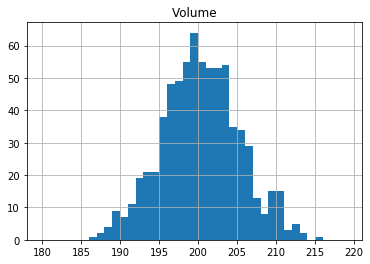
\includegraphics[width=0.6\textwidth]{figures/Untitled_40_1.png}
\end{figure}
%    { \hspace*{\fill} \\}

\begin{tcolorbox}[breakable, size=fbox, boxrule=1pt, pad at break*=1mm,colback=cellbackground, colframe=cellborder]
\begin{Verbatim}[commandchars=\\\{\}]
\PY{n}{df1}\PY{p}{[}\PY{l+s+s1}{\PYZsq{}}\PY{l+s+s1}{Volume}\PY{l+s+s1}{\PYZsq{}}\PY{p}{]} \PY{o}{=} \PY{p}{(}\PY{n}{df1}\PY{p}{[}\PY{l+s+s1}{\PYZsq{}}\PY{l+s+s1}{Volume}\PY{l+s+s1}{\PYZsq{}}\PY{p}{]} \PY{o}{\PYZhy{}} \PY{n}{df1}\PY{p}{[}\PY{l+s+s1}{\PYZsq{}}\PY{l+s+s1}{Volume}\PY{l+s+s1}{\PYZsq{}}\PY{p}{]}\PY{o}{.}\PY{n}{mean}\PY{p}{(}\PY{p}{)}\PY{p}{)} \PY{o}{/} \PY{n}{df1}\PY{p}{[}\PY{l+s+s1}{\PYZsq{}}\PY{l+s+s1}{Volume}\PY{l+s+s1}{\PYZsq{}}\PY{p}{]}\PY{o}{.}\PY{n}{std}\PY{p}{(}\PY{p}{)}

\PY{n}{df1}\PY{o}{.}\PY{n}{hist}\PY{p}{(}\PY{l+s+s1}{\PYZsq{}}\PY{l+s+s1}{Volume}\PY{l+s+s1}{\PYZsq{}}\PY{p}{,} \PY{n}{bins}\PY{o}{=}\PY{n}{np}\PY{o}{.}\PY{n}{arange}\PY{p}{(}\PY{o}{\PYZhy{}}\PY{l+m+mi}{5}\PY{p}{,} \PY{l+m+mi}{5}\PY{p}{,} \PY{l+m+mf}{0.1}\PY{p}{)}\PY{p}{)}
\PY{n+nb}{print} \PY{p}{(}\PY{n}{df1}\PY{p}{[}\PY{l+s+s1}{\PYZsq{}}\PY{l+s+s1}{Volume}\PY{l+s+s1}{\PYZsq{}}\PY{p}{]}\PY{o}{.}\PY{n}{mean}\PY{p}{(}\PY{p}{)}\PY{p}{)}
\PY{n+nb}{print} \PY{p}{(}\PY{n}{df1}\PY{p}{[}\PY{l+s+s1}{\PYZsq{}}\PY{l+s+s1}{Volume}\PY{l+s+s1}{\PYZsq{}}\PY{p}{]}\PY{o}{.}\PY{n}{std}\PY{p}{(}\PY{p}{)}\PY{p}{)}

-6.148550054609154e-15
1.0
\end{Verbatim}
\end{tcolorbox}

\begin{figure}[h]
\centering
  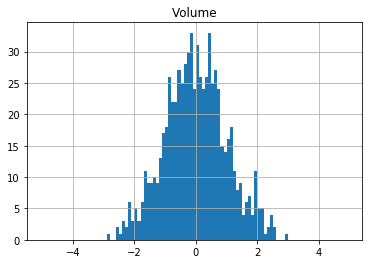
\includegraphics[width=0.6\textwidth]{figures/Untitled_41_1.png}
\end{figure}
  %  { \hspace*{\fill} \\}
    
\clearpage
\section{Plotting in \texttt{python}}\label{plotting-in-python}

As we have just seen \texttt{pandas} allows to quickly draw histograms of dataframe columns, but during an analysis we may want to plot distributions from \texttt{list} or objects not stored in a dataframe. Furthermore the simple although very useful interface doesn't grant full access to all histogram features that we need to produce nice and informative plots.

In order to do so we can use the \texttt{matplotlib} module which is specifically dedicated to plotting (pandas interface is based on the same module indeed). 

In the next Sections we will look briefly to its capabilities. For those interested a more detailed and comprehensive documentation can be found at~\cite{matplotlib}.

\subsection{Canvas}\label{canvas}

The first element we need to plot is a \emph{canvas}, the white
rectangular space where we draw our data. \(\tt{Matplotlib}\) provides a
default canvas if no specific command is given (a 640x480 pixels space)
but you can customize it by specifying many different parameters, the
most commonly are:

\begin{itemize}
	\tightlist
	\item
	\(\tt{figsize}\): width, height in inches. If not provided, defaults
	to \([6.4, 4.8]\);
	\item
	\(\tt{dpi}\): resolution of the figure. If not provided, defaults to
	100;
	\item
	\(\tt{facecolor}\): the background color. If not provided, defaults to
	\(\tt{'white'}\), or \(\tt{'w'}\).
\end{itemize}

In the following example we create a canvas (8 inches x 5 inches) with a
resolution of 80 dots per inches (dpi) and a green background color.

\begin{tcolorbox}[breakable, size=fbox, boxrule=1pt, pad at break*=1mm,colback=cellbackground, colframe=cellborder]
\begin{Verbatim}[commandchars=\\\{\}]
\PY{k+kn}{from} \PY{n+nn}{matplotlib} \PY{k}{import} \PY{n}{pyplot} \PY{k}{as} \PY{n}{plt}
\PY{n}{fig} \PY{o}{=} \PY{n}{plt}\PY{o}{.}\PY{n}{figure}\PY{p}{(}\PY{n}{figsize}\PY{o}{=}\PY{p}{(}\PY{l+m+mi}{8}\PY{p}{,}\PY{l+m+mi}{5}\PY{p}{)}\PY{p}{,} \PY{n}{dpi}\PY{o}{=}\PY{l+m+mi}{80}\PY{p}{,} \PY{n}{facecolor}\PY{o}{=}\PY{l+s+s1}{\PYZsq{}}\PY{l+s+s1}{green}\PY{l+s+s1}{\PYZsq{}}\PY{p}{)}
\end{Verbatim}
\end{tcolorbox}

Once we have a canvas we cannot even draw it unless we a some plot to
show. So let's see the most used type of plots we can use.

\subsection{Chart Object}\label{chart-object}

Below a concise list of the main chart objects that are commonly used
when presenting financial data.

\subsubsection{Histograms}\label{histograms}

A histogram is an approximate representation of the distribution of
numerical data. To construct a histogram, the first step is to \emph{bin}
(or \emph{bucket}) the range of values (i.e. divide the entire range of
values into a series of intervals) and then count how many values fall
into each interval.

If the bins are of equal size, a rectangle is erected over the bin with
height proportional to the frequency (i.e. the number of cases in each
bin).

However, bins need not be of equal width; in that case, the erected
rectangle is defined to have its area proportional to the frequency of
cases in the bin. The vertical axis is then not the frequency but
frequency density (i.e. the number of cases per unit of the variable on
the horizontal axis).

To create an histogram with \(\tt{matplotlib}\) it is enough to pass the
a list (or a \(\tt{numpy.array}\)) with data to represent to the
function \(\tt{hist}\) and then call \(\tt{show()}\) to actually draw
the plot (I have also used the previously defined canvas just to show
the results).

\begin{tcolorbox}[breakable, size=fbox, boxrule=1pt, pad at break*=1mm,colback=cellbackground, colframe=cellborder]
\begin{Verbatim}[commandchars=\\\{\}]
\PY{n}{y1} \PY{o}{=} \PY{p}{[}\PY{l+m+mf}{40.9}\PY{p}{,} \PY{l+m+mf}{49.6}\PY{p}{,} \PY{l+m+mf}{36.5}\PY{p}{,} \PY{l+m+mf}{43.7}\PY{p}{,} \PY{l+m+mf}{52.4}\PY{p}{,} \PY{l+m+mf}{37.0}\PY{p}{,} \PY{l+m+mf}{42.4}\PY{p}{,} \PY{l+m+mf}{38.4}\PY{p}{,} \PY{l+m+mf}{39.9}\PY{p}{,} \PY{l+m+mf}{40.6}\PY{p}{,} \PY{l+m+mf}{35.7}\PY{p}{,} \PY{l+m+mf}{42.4}\PY{p}{,} 
\PY{l+m+mf}{47.7}\PY{p}{,} \PY{l+m+mf}{40.6}\PY{p}{,} \PY{l+m+mf}{47.6}\PY{p}{,} \PY{l+m+mf}{38.3}\PY{p}{,} \PY{l+m+mf}{43.6}\PY{p}{,} \PY{l+m+mf}{38.5}\PY{p}{,} \PY{l+m+mf}{43.5}\PY{p}{,} \PY{l+m+mf}{42.9}\PY{p}{,} \PY{l+m+mf}{42.1}\PY{p}{,} \PY{l+m+mf}{39.8}\PY{p}{,} \PY{l+m+mf}{35.8}\PY{p}{,} \PY{l+m+mf}{44.1}\PY{p}{,} 
\PY{l+m+mf}{43.0}\PY{p}{,} \PY{l+m+mf}{45.4}\PY{p}{,} \PY{l+m+mf}{52.3}\PY{p}{,} \PY{l+m+mf}{41.5}\PY{p}{,} \PY{l+m+mf}{42.6}\PY{p}{,} \PY{l+m+mf}{45.4}\PY{p}{,} \PY{l+m+mf}{38.6}\PY{p}{,} \PY{l+m+mf}{37.3}\PY{p}{,} \PY{l+m+mf}{37.8}\PY{p}{,} \PY{l+m+mf}{48.1}\PY{p}{,} \PY{l+m+mf}{44.8}\PY{p}{,} \PY{l+m+mf}{32.7}\PY{p}{,} 
\PY{l+m+mf}{42.3}\PY{p}{,} \PY{l+m+mf}{33.8}\PY{p}{,} \PY{l+m+mf}{43.1}\PY{p}{,} \PY{l+m+mf}{40.3}\PY{p}{]}
	
\PY{n}{fig} \PY{o}{=} \PY{n}{plt}\PY{o}{.}\PY{n}{figure}\PY{p}{(}\PY{n}{figsize}\PY{o}{=}\PY{p}{(}\PY{l+m+mi}{8}\PY{p}{,}\PY{l+m+mi}{5}\PY{p}{)}\PY{p}{,} \PY{n}{dpi}\PY{o}{=}\PY{l+m+mi}{80}\PY{p}{,} \PY{n}{facecolor}\PY{o}{=}\PY{l+s+s1}{\PYZsq{}}\PY{l+s+s1}{green}\PY{l+s+s1}{\PYZsq{}}\PY{p}{)}
\PY{n}{plt}\PY{o}{.}\PY{n}{hist}\PY{p}{(}\PY{n}{y1}\PY{p}{)}
\PY{n}{plt}\PY{o}{.}\PY{n}{show}\PY{p}{(}\PY{p}{)}
\end{Verbatim}
\end{tcolorbox}

\begin{figure}[h]
	\centering
	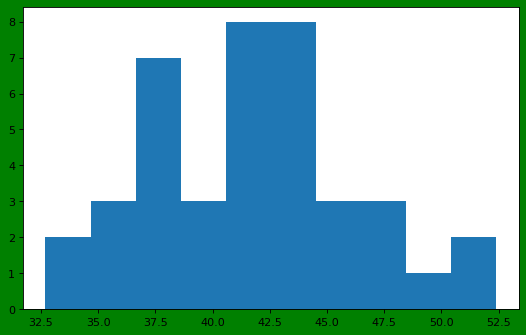
\includegraphics[width=0.7\textwidth]{figures/matplotlib_3_0.png}
\end{figure}

If you are not satisfied with the default binning and/or you want to
change the range shown in the plot, those can be specified in the call
to \(\tt{hist}\) like this

\begin{tcolorbox}[breakable, size=fbox, boxrule=1pt, pad at break*=1mm,colback=cellbackground, colframe=cellborder]
\begin{Verbatim}[commandchars=\\\{\}]
\PY{c+c1}{\PYZsh{} after data there is the number of equally spaced bins}
\PY{c+c1}{\PYZsh{} to be used, then the range}
\PY{n}{plt}\PY{o}{.}\PY{n}{hist}\PY{p}{(}\PY{n}{y}\PY{p}{,} \PY{l+m+mi}{50}\PY{p}{,} \PY{n+nb}{range}\PY{o}{=}\PY{p}{(}\PY{l+m+mi}{30}\PY{p}{,} \PY{l+m+mi}{50}\PY{p}{)}\PY{p}{)}
\PY{n}{plt}\PY{o}{.}\PY{n}{show}\PY{p}{(}\PY{p}{)}
\end{Verbatim}
\end{tcolorbox}

\begin{figure}[h]
	\centering
	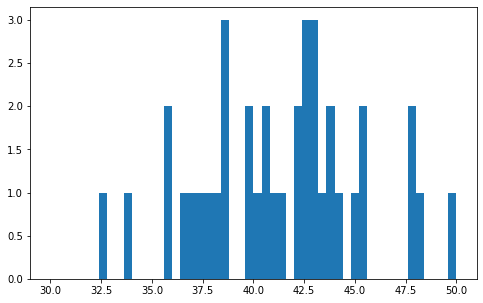
\includegraphics[width=0.7\textwidth]{figures/matplotlib_5_0.png}
\end{figure}

Passing other parameters it is possible to modify the style of the
histogram, like its color. Colors can be specified by their names. For
the basic built-in colors, you can use a single letter

\begin{itemize}
	\tightlist
	\item
	b: blue
	\item
	g: green
	\item
	r: red
	\item
	c: cyan
	\item
	m: magenta
	\item
	y: yellow
	\item
	k: black
	\item
	w: white
\end{itemize}

Plotting multiple histograms on the same canvas is as easy as calling
various times \(\tt{hist}\) (binning should be the same for each
histogram).

To each object that is plotted can be associated a label, passing the
corresponding parameter to the object call, so that we can build a
legend. Latex symbols can be used whenever text is used, the characters
have to enclosed between dollar symbols (i.e. \$\\mu\$). Legend that
will be shown on the canvas with the command \(\tt{legend()}\).

A grid can be added to the plot with \(\tt{plt.grid(True)}\) for a nicer
look.

\begin{tcolorbox}[breakable, size=fbox, boxrule=1pt, pad at break*=1mm,colback=cellbackground, colframe=cellborder]
\begin{Verbatim}[commandchars=\\\{\}]
\PY{n}{y2} \PY{o}{=} \PY{p}{[}\PY{l+m+mf}{40.6}\PY{p}{,} \PY{l+m+mf}{40.5}\PY{p}{,} \PY{l+m+mf}{37.3}\PY{p}{,} \PY{l+m+mf}{37.6}\PY{p}{,} \PY{l+m+mf}{39.0}\PY{p}{,} \PY{l+m+mf}{38.5}\PY{p}{,} \PY{l+m+mf}{36.0}\PY{p}{,} \PY{l+m+mf}{39.0}\PY{p}{,} \PY{l+m+mf}{36.8}\PY{p}{,} \PY{l+m+mf}{41.4}\PY{p}{,} \PY{l+m+mf}{41.9}\PY{p}{,} \PY{l+m+mf}{39.9}\PY{p}{,} 
\PY{l+m+mf}{39.0}\PY{p}{,} \PY{l+m+mf}{37.7}\PY{p}{,} \PY{l+m+mf}{35.0}\PY{p}{,} \PY{l+m+mf}{37.9}\PY{p}{,} \PY{l+m+mf}{35.2}\PY{p}{,} \PY{l+m+mf}{39.5}\PY{p}{,} \PY{l+m+mf}{37.7}\PY{p}{,} \PY{l+m+mf}{38.4}\PY{p}{,} \PY{l+m+mf}{42.4}\PY{p}{,} \PY{l+m+mf}{38.1}\PY{p}{,} \PY{l+m+mf}{39.0}\PY{p}{,} \PY{l+m+mf}{34.7}\PY{p}{,} 
\PY{l+m+mf}{37.1}\PY{p}{,} \PY{l+m+mf}{36.6}\PY{p}{,} \PY{l+m+mf}{37.0}\PY{p}{,} \PY{l+m+mf}{40.8}\PY{p}{,} \PY{l+m+mf}{39.0}\PY{p}{,} \PY{l+m+mf}{41.5}\PY{p}{]}
	
\PY{n}{plt}\PY{o}{.}\PY{n}{hist}\PY{p}{(}\PY{n}{y1}\PY{p}{,} \PY{l+m+mi}{50}\PY{p}{,} \PY{n+nb}{range}\PY{o}{=}\PY{p}{(}\PY{l+m+mi}{30}\PY{p}{,} \PY{l+m+mi}{50}\PY{p}{)}\PY{p}{,} \PY{n}{color}\PY{o}{=}\PY{l+s+s1}{\PYZsq{}}\PY{l+s+s1}{red}\PY{l+s+s1}{\PYZsq{}}\PY{p}{,} \PY{n}{label}\PY{o}{=}\PY{l+s+s1}{\PYZsq{}}\PY{l+s+s1}{Red Hist}\PY{l+s+s1}{\PYZsq{}}\PY{p}{)}
\PY{n}{plt}\PY{o}{.}\PY{n}{hist}\PY{p}{(}\PY{n}{y2}\PY{p}{,} \PY{l+m+mi}{50}\PY{p}{,} \PY{n+nb}{range}\PY{o}{=}\PY{p}{(}\PY{l+m+mi}{30}\PY{p}{,} \PY{l+m+mi}{50}\PY{p}{)}\PY{p}{,} \PY{n}{color}\PY{o}{=}\PY{l+s+s1}{\PYZsq{}}\PY{l+s+s1}{yellow}\PY{l+s+s1}{\PYZsq{}}\PY{p}{,} \PY{n}{label}\PY{o}{=}\PY{l+s+s1}{\PYZsq{}}\PY{l+s+s1}{Yellow Hist}\PY{l+s+s1}{\PYZsq{}}\PY{p}{)}
\PY{n}{plt}\PY{o}{.}\PY{n}{legend}\PY{p}{(}\PY{p}{)}
\PY{n}{plt}\PY{o}{.}\PY{n}{grid}\PY{p}{(}\PY{k+kc}{True}\PY{p}{)}
\PY{n}{plt}\PY{o}{.}\PY{n}{show}\PY{p}{(}\PY{p}{)}
\end{Verbatim}
\end{tcolorbox}

\begin{figure}[h]
	\centering
	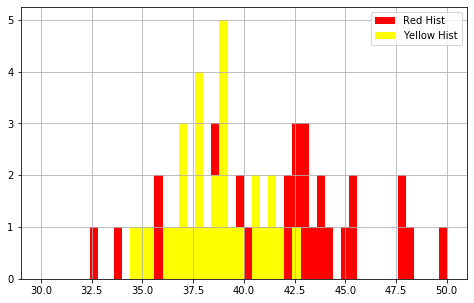
\includegraphics[width=0.7\textwidth]{figures/matplotlib_7_0.png}
\end{figure}

\subsubsection{Scatter Plot}\label{scatter}

A scatter plot is a type of plot using Cartesian coordinates to display
values for typically two variables for a set of data. If the points are
coded (color/shape/size), one additional variable can be displayed.

The data are displayed as a collection of points, each having the value
of one variable determining the position on the horizontal axis and the
value of the other variable determining the position on the vertical
axis.

To create such an object it is enough to call \(\tt{scatter}\) and pass
the \(x\) and \(y\) lists .

\begin{tcolorbox}[breakable, size=fbox, boxrule=1pt, pad at break*=1mm,colback=cellbackground, colframe=cellborder]
\begin{Verbatim}[commandchars=\\\{\}]
\PY{n}{y1} \PY{o}{=} \PY{p}{[}\PY{l+m+mf}{26.2}\PY{p}{,} \PY{l+m+mf}{5.4}\PY{p}{,} \PY{l+m+mf}{7.7}\PY{p}{,} \PY{l+m+mf}{3.8}\PY{p}{,} \PY{l+m+mf}{24.7}\PY{p}{,} \PY{o}{\PYZhy{}}\PY{l+m+mf}{5.5}\PY{p}{,} \PY{l+m+mf}{36.4}\PY{p}{,} \PY{l+m+mf}{12.9}\PY{p}{,} \PY{l+m+mf}{25.2}\PY{p}{,} \PY{l+m+mf}{21.0}\PY{p}{,} \PY{l+m+mf}{39.6}\PY{p}{,} 
\PY{l+m+mf}{5.9}\PY{p}{,} \PY{l+m+mf}{24.8}\PY{p}{,} \PY{l+m+mf}{25.7}\PY{p}{,} \PY{l+m+mf}{42.3}\PY{p}{,} \PY{l+m+mf}{21.5}\PY{p}{,} \PY{l+m+mf}{32.3}\PY{p}{,} \PY{l+m+mf}{26.7}\PY{p}{,} \PY{l+m+mf}{37.4}\PY{p}{,} \PY{l+m+mf}{44.3}\PY{p}{,} \PY{l+m+mf}{29.0}\PY{p}{,} 
\PY{l+m+mf}{52.9}\PY{p}{,} \PY{l+m+mf}{52.0}\PY{p}{,} \PY{l+m+mf}{49.5}\PY{p}{,} \PY{l+m+mf}{55.0}\PY{p}{,} \PY{l+m+mf}{40.7}\PY{p}{,} \PY{l+m+mf}{47.8}\PY{p}{,} \PY{l+m+mf}{41.1}\PY{p}{,} \PY{l+m+mf}{49.3}\PY{p}{,} \PY{l+m+mf}{58.8}\PY{p}{,} \PY{l+m+mf}{48.1}\PY{p}{,} 
\PY{l+m+mf}{52.5}\PY{p}{,} \PY{l+m+mf}{51.1}\PY{p}{,} \PY{l+m+mf}{51.0}\PY{p}{,} \PY{l+m+mf}{54.3}\PY{p}{,} \PY{l+m+mf}{62.4}\PY{p}{,} \PY{l+m+mf}{52.8}\PY{p}{,} \PY{l+m+mf}{67.8}\PY{p}{,} \PY{l+m+mf}{83.6}\PY{p}{,} \PY{l+m+mf}{75.9}\PY{p}{]}
	
\PY{n}{x} \PY{o}{=} \PY{n+nb}{range}\PY{p}{(}\PY{n+nb}{len}\PY{p}{(}\PY{n}{y1}\PY{p}{)}\PY{p}{)}
\PY{n}{plt}\PY{o}{.}\PY{n}{scatter}\PY{p}{(}\PY{n}{x}\PY{p}{,} \PY{n}{y1}\PY{p}{)}
\PY{n}{plt}\PY{o}{.}\PY{n}{show}\PY{p}{(}\PY{p}{)}
\end{Verbatim}
\end{tcolorbox}

\begin{figure}[h]
	\centering
	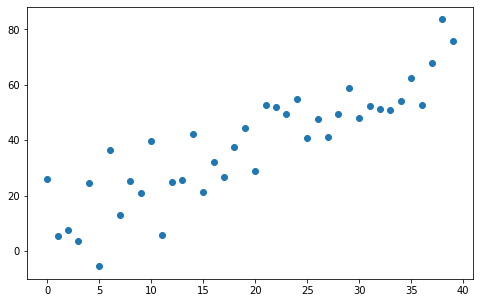
\includegraphics[width=0.7\textwidth]{figures/matplotlib_9_0.png}
\end{figure}

Other parameters can be passes to \(\tt{scatter}\) the most useful are

\begin{itemize}
	\tightlist
	\item
	\(\tt{label}\): label the scatter plot fot the legend;
	\item
	\(\tt{color}\): set the color of the marker;
	\item
	\(\tt{marker}\): set the sityle of the marker defined with a single
	character (+,*, o, x\ldots{});
	\item
	\(\tt{s=}\): set the size of the marker.
\end{itemize}

And of course multiple scatter plot can be shown together in the same
canvas calling \(\tt{scatter}\) accordingly.

\begin{tcolorbox}[breakable, size=fbox, boxrule=1pt, pad at break*=1mm,colback=cellbackground, colframe=cellborder]
\begin{Verbatim}[commandchars=\\\{\}]
\PY{n}{y2} \PY{o}{=} \PY{p}{[}\PY{l+m+mf}{22.2}\PY{p}{,} \PY{l+m+mf}{3.4}\PY{p}{,} \PY{l+m+mf}{7.7}\PY{p}{,} \PY{l+m+mf}{5.8}\PY{p}{,} \PY{l+m+mf}{28.7}\PY{p}{,} \PY{l+m+mf}{0.5}\PY{p}{,} \PY{l+m+mf}{44.4}\PY{p}{,} \PY{l+m+mf}{22.9}\PY{p}{,} \PY{l+m+mf}{37.2}\PY{p}{,} \PY{l+m+mf}{35.0}\PY{p}{,} \PY{l+m+mf}{55.6}\PY{p}{,} 
\PY{l+m+mf}{23.9}\PY{p}{,} \PY{l+m+mf}{44.8}\PY{p}{,} \PY{l+m+mf}{47.7}\PY{p}{,} \PY{l+m+mf}{66.3}\PY{p}{,} \PY{l+m+mf}{47.5}\PY{p}{,} \PY{l+m+mf}{60.3}\PY{p}{,} \PY{l+m+mf}{56.7}\PY{p}{,} \PY{l+m+mf}{69.4}\PY{p}{,} \PY{l+m+mf}{78.3}\PY{p}{,} \PY{l+m+mf}{65.0}\PY{p}{,} 
\PY{l+m+mf}{90.9}\PY{p}{,} \PY{l+m+mf}{92.0}\PY{p}{,} \PY{l+m+mf}{91.5}\PY{p}{,} \PY{l+m+mf}{99.0}\PY{p}{,} \PY{l+m+mf}{86.7}\PY{p}{,} \PY{l+m+mf}{95.8}\PY{p}{,} \PY{l+m+mf}{91.1}\PY{p}{,} \PY{l+m+mf}{101.3}\PY{p}{,} \PY{l+m+mf}{112.8}\PY{p}{,} 
\PY{l+m+mf}{104.1}\PY{p}{,} \PY{l+m+mf}{110.5}\PY{p}{,} \PY{l+m+mf}{111.1}\PY{p}{,} \PY{l+m+mf}{113.0}\PY{p}{,} \PY{l+m+mf}{118.3}\PY{p}{,} \PY{l+m+mf}{128.4}\PY{p}{,} \PY{l+m+mf}{120.8}\PY{p}{,} \PY{l+m+mf}{137.8}\PY{p}{,} \PY{l+m+mf}{155.6}\PY{p}{,} \PY{l+m+mf}{149.9}\PY{p}{]}
	
\PY{n}{plt}\PY{o}{.}\PY{n}{scatter}\PY{p}{(}\PY{n+nb}{range}\PY{p}{(}\PY{n+nb}{len}\PY{p}{(}\PY{n}{y1}\PY{p}{)}\PY{p}{)}\PY{p}{,} \PY{n}{y1}\PY{p}{,} \PY{n}{s}\PY{o}{=}\PY{l+m+mi}{10}\PY{p}{,} \PY{n}{marker}\PY{o}{=}\PY{l+s+s2}{\PYZdq{}}\PY{l+s+s2}{o}\PY{l+s+s2}{\PYZdq{}}\PY{p}{,} 
            \PY{n}{color}\PY{o}{=}\PY{l+s+s2}{\PYZdq{}}\PY{l+s+s2}{lightblue}\PY{l+s+s2}{\PYZdq{}}\PY{p}{,} \PY{n}{label}\PY{o}{=}\PY{l+s+s2}{\PYZdq{}}\PY{l+s+s2}{1st Scatter}\PY{l+s+s2}{\PYZdq{}}\PY{p}{)}
\PY{n}{plt}\PY{o}{.}\PY{n}{scatter}\PY{p}{(}\PY{n+nb}{range}\PY{p}{(}\PY{n+nb}{len}\PY{p}{(}\PY{n}{y2}\PY{p}{)}\PY{p}{)}\PY{p}{,} \PY{n}{y2}\PY{p}{,} \PY{n}{s}\PY{o}{=}\PY{l+m+mi}{30}\PY{p}{,} \PY{n}{marker}\PY{o}{=}\PY{l+s+s2}{\PYZdq{}}\PY{l+s+s2}{*}\PY{l+s+s2}{\PYZdq{}}\PY{p}{,} 
            \PY{n}{color}\PY{o}{=}\PY{l+s+s2}{\PYZdq{}}\PY{l+s+s2}{brown}\PY{l+s+s2}{\PYZdq{}}\PY{p}{,} \PY{n}{label}\PY{o}{=}\PY{l+s+s2}{\PYZdq{}}\PY{l+s+s2}{2nd Scatter}\PY{l+s+s2}{\PYZdq{}}\PY{p}{)}
\PY{n}{plt}\PY{o}{.}\PY{n}{legend}\PY{p}{(}\PY{p}{)}
\PY{n}{plt}\PY{o}{.}\PY{n}{show}\PY{p}{(}\PY{p}{)}
\end{Verbatim}
\end{tcolorbox}

\begin{figure}[h]
	\centering
	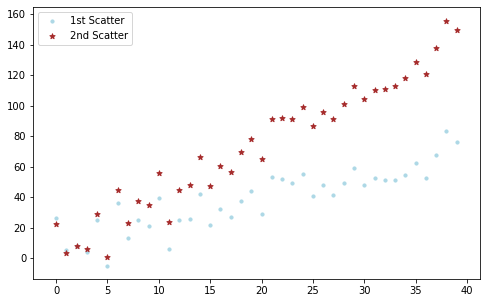
\includegraphics[width=0.65\textwidth]{figures/matplotlib_11_0.png}
\end{figure}

\subsubsection{Plot}\label{plot}

If you want to still plot \(x\) and \(y\) points but they should be
connected with a line you can use the function \(\tt{plot}\). It acts
similarly to \(\tt{scatter}\) but the graphical result will be
different.

For example below the same two scatter plots of the previous example are
plotted with \(\tt{plot}\)

\begin{tcolorbox}[breakable, size=fbox, boxrule=1pt, pad at break*=1mm,colback=cellbackground, colframe=cellborder]
\begin{Verbatim}[commandchars=\\\{\}]
\PY{n}{plt}\PY{o}{.}\PY{n}{plot}\PY{p}{(}\PY{n}{x}\PY{p}{,} \PY{n}{y1}\PY{p}{,} \PY{n}{label}\PY{o}{=}\PY{l+s+s2}{\PYZdq{}}\PY{l+s+s2}{1st Plot}\PY{l+s+s2}{\PYZdq{}}\PY{p}{)}
\PY{n}{plt}\PY{o}{.}\PY{n}{plot}\PY{p}{(}\PY{n}{x}\PY{p}{,} \PY{n}{y2}\PY{p}{,} \PY{n}{label}\PY{o}{=}\PY{l+s+s2}{\PYZdq{}}\PY{l+s+s2}{2nd Plot}\PY{l+s+s2}{\PYZdq{}}\PY{p}{)}
\PY{n}{plt}\PY{o}{.}\PY{n}{legend}\PY{p}{(}\PY{p}{)}
\PY{n}{plt}\PY{o}{.}\PY{n}{show}\PY{p}{(}\PY{p}{)}
\end{Verbatim}
\end{tcolorbox}

\begin{figure}[h]
	\centering
	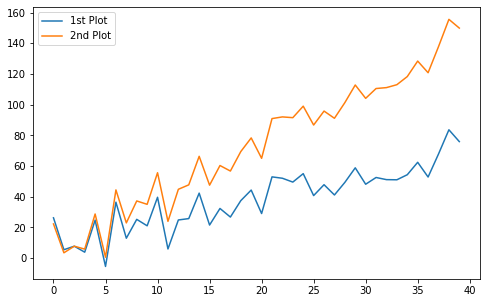
\includegraphics[width=0.65\textwidth]{figures/matplotlib_13_0.png}
\end{figure}

In this case the parameters the parameters allow to control the line
style and the possibility to add the marker at each point

\begin{itemize}
	\tightlist
	\item
	\(\tt{label}\): label the scatter plot fot the legend;
	\item
	\(\tt{color}\): set the color of the marker and the line;
	\item
	\(\tt{marker}\): set the sityle of the marker defined with a single
	character (+,*, o, x\ldots{});
	\item
	\(\tt{s}\): set the size of the marker;
	\item
	\(\tt{linestyle}\): style of the line (`-', `--', `-.', `:');
	\item
	\(\tt{linewidth}\): thickness of the line.
\end{itemize}

\begin{tcolorbox}[breakable, size=fbox, boxrule=1pt, pad at break*=1mm,colback=cellbackground, colframe=cellborder]
\begin{Verbatim}[commandchars=\\\{\}]
\PY{n}{plt}\PY{o}{.}\PY{n}{plot}\PY{p}{(}\PY{n}{x}\PY{p}{,} \PY{n}{y1}\PY{p}{,} \PY{n}{marker}\PY{o}{=}\PY{l+s+s2}{\PYZdq{}}\PY{l+s+s2}{+}\PY{l+s+s2}{\PYZdq{}}\PY{p}{,} \PY{n}{linestyle}\PY{o}{=}\PY{l+s+s2}{\PYZdq{}}\PY{l+s+s2}{:}\PY{l+s+s2}{\PYZdq{}}\PY{p}{,} \PY{n}{color}\PY{o}{=}\PY{l+s+s2}{\PYZdq{}}\PY{l+s+s2}{darkgreen}\PY{l+s+s2}{\PYZdq{}}\PY{p}{,} \PY{n}{label}\PY{o}{=}\PY{l+s+s2}{\PYZdq{}}\PY{l+s+s2}{1st Plot}\PY{l+s+s2}{\PYZdq{}}\PY{p}{)}
\PY{n}{plt}\PY{o}{.}\PY{n}{plot}\PY{p}{(}\PY{n}{x}\PY{p}{,} \PY{n}{y2}\PY{p}{,} \PY{n}{marker}\PY{o}{=}\PY{l+s+s2}{\PYZdq{}}\PY{l+s+s2}{x}\PY{l+s+s2}{\PYZdq{}}\PY{p}{,} \PY{n}{linewidth}\PY{o}{=}\PY{l+m+mi}{5}\PY{p}{,} \PY{n}{color}\PY{o}{=}\PY{l+s+s2}{\PYZdq{}}\PY{l+s+s2}{pink}\PY{l+s+s2}{\PYZdq{}}\PY{p}{,} \PY{n}{label}\PY{o}{=}\PY{l+s+s2}{\PYZdq{}}\PY{l+s+s2}{2nd Plot}\PY{l+s+s2}{\PYZdq{}}\PY{p}{)}
\PY{n}{plt}\PY{o}{.}\PY{n}{legend}\PY{p}{(}\PY{p}{)}
\PY{n}{plt}\PY{o}{.}\PY{n}{show}\PY{p}{(}\PY{p}{)}
\end{Verbatim}
\end{tcolorbox}

\begin{figure}[h]
	\centering
	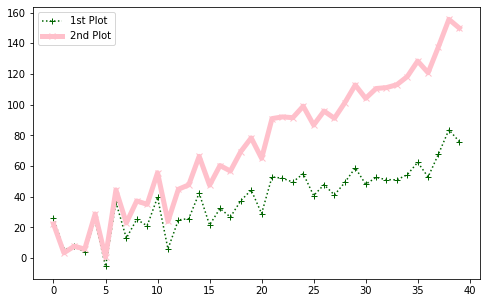
\includegraphics[width=0.7\textwidth]{figures/matplotlib_15_0.png}
\end{figure}

\subsubsection{Plotting a Function}\label{plotting-a-function}

Functions can be plotted using the \(\tt{plot}\) method. They can be
functions from \(\tt{python}\) modules or user-defined.

As an example let's try to plot \(\mathrm{sin}(x/2)\), in the example we
will use \(\tt{numpy.arange}\) function which extend the functionalities
of the standard \(\tt{range}\) allowing for non integer steps.

In such cases it is always recommended to use \(\tt{numpy}\) functions
and not those defined in \(\tt{math}\) since they also accept arrays in
input for a faster processing (i.e.~it is not need to loop over each
\(x\) value to compute the value function since it is done
automatically).

\begin{tcolorbox}[breakable, size=fbox, boxrule=1pt, pad at break*=1mm,colback=cellbackground, colframe=cellborder]
\begin{Verbatim}[commandchars=\\\{\}]
\PY{k+kn}{from} \PY{n+nn}{numpy} \PY{k}{import} \PY{n}{arange}\PY{p}{,} \PY{n}{sin}
	
\PY{k}{def} \PY{n+nf}{func}\PY{p}{(}\PY{n}{x}\PY{p}{)}\PY{p}{:}
    \PY{k}{return} \PY{n}{sin}\PY{p}{(}\PY{n}{x}\PY{o}{/}\PY{l+m+mi}{2}\PY{p}{)}
	
\PY{n}{xs} \PY{o}{=} \PY{n}{arange}\PY{p}{(}\PY{o}{\PYZhy{}}\PY{l+m+mi}{10}\PY{p}{,} \PY{l+m+mi}{10}\PY{p}{,} \PY{l+m+mf}{0.01}\PY{p}{)}
	
\PY{n}{fig} \PY{o}{=} \PY{n}{plt}\PY{o}{.}\PY{n}{figure}\PY{p}{(}\PY{n}{figsize}\PY{o}{=}\PY{p}{(}\PY{l+m+mi}{8}\PY{p}{,}\PY{l+m+mi}{5}\PY{p}{)}\PY{p}{)}
\PY{n}{plt}\PY{o}{.}\PY{n}{plot}\PY{p}{(}\PY{n}{xs}\PY{p}{,} \PY{n}{func}\PY{p}{(}\PY{n}{xs}\PY{p}{)}\PY{p}{)}
\PY{n}{plt}\PY{o}{.}\PY{n}{show}\PY{p}{(}\PY{p}{)}
\end{Verbatim}
\end{tcolorbox}

\begin{figure}[h]
	\centering
	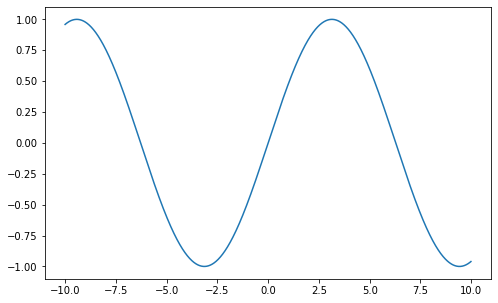
\includegraphics[width=0.65\textwidth]{figures/matplotlib_17_0.png}
\end{figure}

\subsection{Axes}\label{axes}

The axis of a any plot can be formatted with many options.

First of all the axis range can be controlled with
\(\tt{xlim(min, max}\) and \(\tt{ylim(min, max}\). Then labels can be
added with \(\tt{xlabel(myLabel)}\) and \(\tt{ylabel(myLabel)}\). A
global title to the plot can also be specified with
\(\tt{plt.title(myTitle)}\).

Referring to the previous example we can write

\begin{tcolorbox}[breakable, size=fbox, boxrule=1pt, pad at break*=1mm,colback=cellbackground, colframe=cellborder]
\begin{Verbatim}[commandchars=\\\{\}]
\PY{n}{fig} \PY{o}{=} \PY{n}{plt}\PY{o}{.}\PY{n}{figure}\PY{p}{(}\PY{n}{figsize}\PY{o}{=}\PY{p}{(}\PY{l+m+mi}{8}\PY{p}{,}\PY{l+m+mi}{5}\PY{p}{)}\PY{p}{)}
\PY{n}{plt}\PY{o}{.}\PY{n}{plot}\PY{p}{(}\PY{n}{x}\PY{p}{,} \PY{n}{y1}\PY{p}{,} \PY{n}{marker}\PY{o}{=}\PY{l+s+s2}{\PYZdq{}}\PY{l+s+s2}{+}\PY{l+s+s2}{\PYZdq{}}\PY{p}{,} \PY{n}{linestyle}\PY{o}{=}\PY{l+s+s2}{\PYZdq{}}\PY{l+s+s2}{:}\PY{l+s+s2}{\PYZdq{}}\PY{p}{,} \PY{n}{color}\PY{o}{=}\PY{l+s+s2}{\PYZdq{}}\PY{l+s+s2}{darkgreen}\PY{l+s+s2}{\PYZdq{}}\PY{p}{,} \PY{n}{label}\PY{o}{=}\PY{l+s+s2}{\PYZdq{}}\PY{l+s+s2}{1st Plot}\PY{l+s+s2}{\PYZdq{}}\PY{p}{)}
\PY{n}{plt}\PY{o}{.}\PY{n}{plot}\PY{p}{(}\PY{n}{x}\PY{p}{,} \PY{n}{y2}\PY{p}{,} \PY{n}{marker}\PY{o}{=}\PY{l+s+s2}{\PYZdq{}}\PY{l+s+s2}{x}\PY{l+s+s2}{\PYZdq{}}\PY{p}{,} \PY{n}{linewidth}\PY{o}{=}\PY{l+m+mi}{5}\PY{p}{,} \PY{n}{color}\PY{o}{=}\PY{l+s+s2}{\PYZdq{}}\PY{l+s+s2}{pink}\PY{l+s+s2}{\PYZdq{}}\PY{p}{,} \PY{n}{label}\PY{o}{=}\PY{l+s+s2}{\PYZdq{}}\PY{l+s+s2}{2nd Plot}\PY{l+s+s2}{\PYZdq{}}\PY{p}{)}
\PY{n}{plt}\PY{o}{.}\PY{n}{title}\PY{p}{(}\PY{l+s+s2}{\PYZdq{}}\PY{l+s+s2}{Plot Title}\PY{l+s+s2}{\PYZdq{}}\PY{p}{)}
\PY{n}{plt}\PY{o}{.}\PY{n}{xlabel}\PY{p}{(}\PY{l+s+s2}{\PYZdq{}}\PY{l+s+s2}{x label}\PY{l+s+s2}{\PYZdq{}}\PY{p}{)}
\PY{n}{plt}\PY{o}{.}\PY{n}{ylabel}\PY{p}{(}\PY{l+s+s2}{\PYZdq{}}\PY{l+s+s2}{y label}\PY{l+s+s2}{\PYZdq{}}\PY{p}{)}
\PY{n}{plt}\PY{o}{.}\PY{n}{legend}\PY{p}{(}\PY{p}{)}
\PY{n}{plt}\PY{o}{.}\PY{n}{show}\PY{p}{(}\PY{p}{)}
\end{Verbatim}
\end{tcolorbox}

\begin{figure}[h]
	\centering
	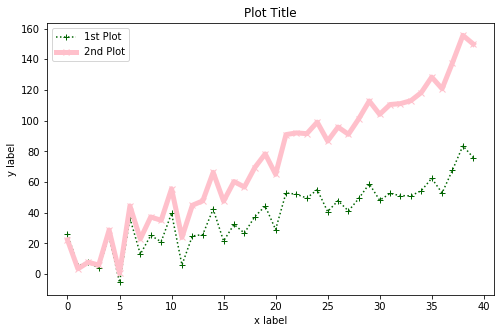
\includegraphics[width=0.65\textwidth]{figures/matplotlib_19_0.png}
\end{figure}

It can also be specified if axis has to be in linear or log scale with
\(\tt{xscale("log")}\) and/or \(\tt{yscale("log")}\).

\begin{tcolorbox}[breakable, size=fbox, boxrule=1pt, pad at break*=1mm,colback=cellbackground, colframe=cellborder]
\begin{Verbatim}[commandchars=\\\{\}]
\PY{n}{fig} \PY{o}{=} \PY{n}{plt}\PY{o}{.}\PY{n}{figure}\PY{p}{(}\PY{n}{figsize}\PY{o}{=}\PY{p}{(}\PY{l+m+mi}{8}\PY{p}{,}\PY{l+m+mi}{5}\PY{p}{)}\PY{p}{)}
\PY{n}{plt}\PY{o}{.}\PY{n}{plot}\PY{p}{(}\PY{n}{x}\PY{p}{,} \PY{n}{y1}\PY{p}{,} \PY{n}{marker}\PY{o}{=}\PY{l+s+s2}{\PYZdq{}}\PY{l+s+s2}{+}\PY{l+s+s2}{\PYZdq{}}\PY{p}{,} \PY{n}{linestyle}\PY{o}{=}\PY{l+s+s2}{\PYZdq{}}\PY{l+s+s2}{:}\PY{l+s+s2}{\PYZdq{}}\PY{p}{,} \PY{n}{color}\PY{o}{=}\PY{l+s+s2}{\PYZdq{}}\PY{l+s+s2}{darkgreen}\PY{l+s+s2}{\PYZdq{}}\PY{p}{,} \PY{n}{label}\PY{o}{=}\PY{l+s+s2}{\PYZdq{}}\PY{l+s+s2}{1st Plot}\PY{l+s+s2}{\PYZdq{}}\PY{p}{)}
\PY{n}{plt}\PY{o}{.}\PY{n}{plot}\PY{p}{(}\PY{n}{x}\PY{p}{,} \PY{n}{y2}\PY{p}{,} \PY{n}{marker}\PY{o}{=}\PY{l+s+s2}{\PYZdq{}}\PY{l+s+s2}{x}\PY{l+s+s2}{\PYZdq{}}\PY{p}{,} \PY{n}{linewidth}\PY{o}{=}\PY{l+m+mi}{5}\PY{p}{,} \PY{n}{color}\PY{o}{=}\PY{l+s+s2}{\PYZdq{}}\PY{l+s+s2}{pink}\PY{l+s+s2}{\PYZdq{}}\PY{p}{,} \PY{n}{label}\PY{o}{=}\PY{l+s+s2}{\PYZdq{}}\PY{l+s+s2}{2nd Plot}\PY{l+s+s2}{\PYZdq{}}\PY{p}{)}
\PY{n}{plt}\PY{o}{.}\PY{n}{title}\PY{p}{(}\PY{l+s+s2}{\PYZdq{}}\PY{l+s+s2}{Plot Title}\PY{l+s+s2}{\PYZdq{}}\PY{p}{)}
\PY{n}{plt}\PY{o}{.}\PY{n}{xlabel}\PY{p}{(}\PY{l+s+s2}{\PYZdq{}}\PY{l+s+s2}{x label}\PY{l+s+s2}{\PYZdq{}}\PY{p}{)}
\PY{n}{plt}\PY{o}{.}\PY{n}{ylabel}\PY{p}{(}\PY{l+s+s2}{\PYZdq{}}\PY{l+s+s2}{y label}\PY{l+s+s2}{\PYZdq{}}\PY{p}{)}
\PY{n}{plt}\PY{o}{.}\PY{n}{xscale}\PY{p}{(}\PY{l+s+s2}{\PYZdq{}}\PY{l+s+s2}{log}\PY{l+s+s2}{\PYZdq{}}\PY{p}{)}
\PY{n}{plt}\PY{o}{.}\PY{n}{yscale}\PY{p}{(}\PY{l+s+s2}{\PYZdq{}}\PY{l+s+s2}{log}\PY{l+s+s2}{\PYZdq{}}\PY{p}{)}
\PY{n}{plt}\PY{o}{.}\PY{n}{legend}\PY{p}{(}\PY{p}{)}
\PY{n}{plt}\PY{o}{.}\PY{n}{show}\PY{p}{(}\PY{p}{)}
\end{Verbatim}
\end{tcolorbox}

\begin{figure}[h]
	\centering
	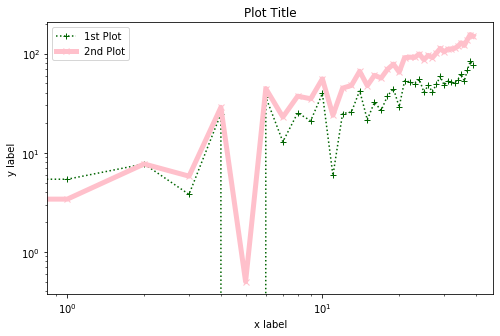
\includegraphics[width=0.7\textwidth]{figures/matplotlib_21_0.png}
\end{figure}

\subsubsection{Date on Axis}\label{date-on-axis}

A special need, very common in finance, is to have dates on the \(x\)
axis. This can be done like shown in the next example:

\begin{tcolorbox}[breakable, size=fbox, boxrule=1pt, pad at break*=1mm,colback=cellbackground, colframe=cellborder]
\begin{Verbatim}[commandchars=\\\{\}]
\PY{k+kn}{import} \PY{n+nn}{datetime} \PY{k}{as} \PY{n+nn}{dt}
\PY{k+kn}{import} \PY{n+nn}{matplotlib}\PY{n+nn}{.}\PY{n+nn}{dates} \PY{k}{as} \PY{n+nn}{mdates}
	
\PY{n}{dates} \PY{o}{=} \PY{p}{[}\PY{l+s+s1}{\PYZsq{}}\PY{l+s+s1}{01/02/1991}\PY{l+s+s1}{\PYZsq{}}\PY{p}{,}\PY{l+s+s1}{\PYZsq{}}\PY{l+s+s1}{01/03/1991}\PY{l+s+s1}{\PYZsq{}}\PY{p}{,}\PY{l+s+s1}{\PYZsq{}}\PY{l+s+s1}{01/04/1991}\PY{l+s+s1}{\PYZsq{}}\PY{p}{]}
\PY{n}{xd} \PY{o}{=} \PY{p}{[}\PY{n}{dt}\PY{o}{.}\PY{n}{datetime}\PY{o}{.}\PY{n}{strptime}\PY{p}{(}\PY{n}{d}\PY{p}{,}\PY{l+s+s1}{\PYZsq{}}\PY{l+s+s1}{\PYZpc{}}\PY{l+s+s1}{m/}\PY{l+s+si}{\PYZpc{}d}\PY{l+s+s1}{/}\PY{l+s+s1}{\PYZpc{}}\PY{l+s+s1}{Y}\PY{l+s+s1}{\PYZsq{}}\PY{p}{)}\PY{o}{.}\PY{n}{date}\PY{p}{(}\PY{p}{)} \PY{k}{for} \PY{n}{d} \PY{o+ow}{in} \PY{n}{dates}\PY{p}{]}
\PY{n}{yd} \PY{o}{=} \PY{n+nb}{range}\PY{p}{(}\PY{n+nb}{len}\PY{p}{(}\PY{n}{xd}\PY{p}{)}\PY{p}{)}
	
\PY{n}{fig} \PY{o}{=} \PY{n}{plt}\PY{o}{.}\PY{n}{figure}\PY{p}{(}\PY{n}{figsize}\PY{o}{=}\PY{p}{(}\PY{l+m+mi}{8}\PY{p}{,}\PY{l+m+mi}{5}\PY{p}{)}\PY{p}{)}
\PY{n}{plt}\PY{o}{.}\PY{n}{gca}\PY{p}{(}\PY{p}{)}\PY{o}{.}\PY{n}{xaxis}\PY{o}{.}\PY{n}{set\PYZus{}major\PYZus{}formatter}\PY{p}{(}\PY{n}{mdates}\PY{o}{.}\PY{n}{DateFormatter}\PY{p}{(}\PY{l+s+s1}{\PYZsq{}}\PY{l+s+s1}{\PYZpc{}}\PY{l+s+s1}{m/}\PY{l+s+si}{\PYZpc{}d}\PY{l+s+s1}{/}\PY{l+s+s1}{\PYZpc{}}\PY{l+s+s1}{Y}\PY{l+s+s1}{\PYZsq{}}\PY{p}{)}\PY{p}{)}
\PY{n}{plt}\PY{o}{.}\PY{n}{gca}\PY{p}{(}\PY{p}{)}\PY{o}{.}\PY{n}{xaxis}\PY{o}{.}\PY{n}{set\PYZus{}major\PYZus{}locator}\PY{p}{(}\PY{n}{mdates}\PY{o}{.}\PY{n}{DayLocator}\PY{p}{(}\PY{p}{)}\PY{p}{)}
\PY{n}{plt}\PY{o}{.}\PY{n}{plot}\PY{p}{(}\PY{n}{xd}\PY{p}{,} \PY{n}{yd}\PY{p}{)}
\PY{n}{plt}\PY{o}{.}\PY{n}{gcf}\PY{p}{(}\PY{p}{)}\PY{o}{.}\PY{n}{autofmt\PYZus{}xdate}\PY{p}{(}\PY{p}{)} \PY{c+c1}{\PYZsh{} this makes a prettier formatting}
\PY{n}{plt}\PY{o}{.}\PY{n}{show}\PY{p}{(}\PY{p}{)}
\end{Verbatim}
\end{tcolorbox}

\begin{figure}[h]
	\centering
	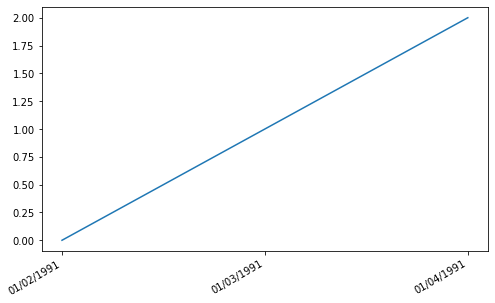
\includegraphics[width=0.6\textwidth]{figures/matplotlib_23_0.png}
\end{figure}

\subsection{Subplots}\label{subplots}

It may happen that we need to plot two or more plots side by side or in
a grid fashion.

The canvas can be then split into subcanvases with the \(\tt{subplot}\)
commands which takes in input the number of rows, columns and the index
of the current subplot. It returns the \emph{subcanvas} object that can
be used to draw like previously shown.

There is one complication though, some of the commands change when
dealing with subplot, \(\tt{xlabel}\) and \(\tt{ylabel}\) for example
becomes \(\tt{set_xlabel}\) and \(\tt{set_ylabel}\). Similarly for
\(\tt{xlim}\) and \(\tt{ylim}\).

As an example imagine that we want to plot the previous plots side by
side on two canvases instead of together in the same

\begin{tcolorbox}[breakable, size=fbox, boxrule=1pt, pad at break*=1mm,colback=cellbackground, colframe=cellborder]
\begin{Verbatim}[commandchars=\\\{\}]
\PY{n}{fig} \PY{o}{=} \PY{n}{plt}\PY{o}{.}\PY{n}{figure}\PY{p}{(}\PY{n}{figsize}\PY{o}{=}\PY{p}{(}\PY{l+m+mi}{8}\PY{p}{,}\PY{l+m+mi}{5}\PY{p}{)}\PY{p}{)}
	
\PY{n}{sub1} \PY{o}{=} \PY{n}{plt}\PY{o}{.}\PY{n}{subplot}\PY{p}{(}\PY{l+m+mi}{1}\PY{p}{,} \PY{l+m+mi}{2}\PY{p}{,} \PY{l+m+mi}{1}\PY{p}{)}
\PY{n}{sub1}\PY{o}{.}\PY{n}{plot}\PY{p}{(}\PY{n}{x}\PY{p}{,} \PY{n}{y1}\PY{p}{,} \PY{n}{marker}\PY{o}{=}\PY{l+s+s2}{\PYZdq{}}\PY{l+s+s2}{+}\PY{l+s+s2}{\PYZdq{}}\PY{p}{,} \PY{n}{linestyle}\PY{o}{=}\PY{l+s+s2}{\PYZdq{}}\PY{l+s+s2}{:}\PY{l+s+s2}{\PYZdq{}}\PY{p}{,} \PY{n}{color}\PY{o}{=}\PY{l+s+s2}{\PYZdq{}}\PY{l+s+s2}{darkgreen}\PY{l+s+s2}{\PYZdq{}}\PY{p}{,} \PY{n}{label}\PY{o}{=}\PY{l+s+s2}{\PYZdq{}}\PY{l+s+s2}{1st Plot}\PY{l+s+s2}{\PYZdq{}}\PY{p}{)}
\PY{n}{sub1}\PY{o}{.}\PY{n}{set\PYZus{}xlabel}\PY{p}{(}\PY{l+s+s2}{\PYZdq{}}\PY{l+s+s2}{x label}\PY{l+s+s2}{\PYZdq{}}\PY{p}{)}
\PY{n}{sub1}\PY{o}{.}\PY{n}{set\PYZus{}ylabel}\PY{p}{(}\PY{l+s+s2}{\PYZdq{}}\PY{l+s+s2}{y label}\PY{l+s+s2}{\PYZdq{}}\PY{p}{)}
\PY{n}{sub1}\PY{o}{.}\PY{n}{legend}\PY{p}{(}\PY{p}{)}
	
\PY{n}{sub2} \PY{o}{=} \PY{n}{plt}\PY{o}{.}\PY{n}{subplot}\PY{p}{(}\PY{l+m+mi}{1}\PY{p}{,} \PY{l+m+mi}{2}\PY{p}{,} \PY{l+m+mi}{2}\PY{p}{)}
\PY{n}{sub2}\PY{o}{.}\PY{n}{plot}\PY{p}{(}\PY{n}{x}\PY{p}{,} \PY{n}{y2}\PY{p}{,} \PY{n}{marker}\PY{o}{=}\PY{l+s+s2}{\PYZdq{}}\PY{l+s+s2}{x}\PY{l+s+s2}{\PYZdq{}}\PY{p}{,} \PY{n}{linewidth}\PY{o}{=}\PY{l+m+mi}{5}\PY{p}{,} \PY{n}{color}\PY{o}{=}\PY{l+s+s2}{\PYZdq{}}\PY{l+s+s2}{pink}\PY{l+s+s2}{\PYZdq{}}\PY{p}{,} \PY{n}{label}\PY{o}{=}\PY{l+s+s2}{\PYZdq{}}\PY{l+s+s2}{2nd Plot}\PY{l+s+s2}{\PYZdq{}}\PY{p}{)}
\PY{n}{sub2}\PY{o}{.}\PY{n}{set\PYZus{}xlabel}\PY{p}{(}\PY{l+s+s2}{\PYZdq{}}\PY{l+s+s2}{x label}\PY{l+s+s2}{\PYZdq{}}\PY{p}{)}
\PY{n}{sub2}\PY{o}{.}\PY{n}{set\PYZus{}ylabel}\PY{p}{(}\PY{l+s+s2}{\PYZdq{}}\PY{l+s+s2}{y label}\PY{l+s+s2}{\PYZdq{}}\PY{p}{)}
\PY{n}{sub2}\PY{o}{.}\PY{n}{legend}\PY{p}{(}\PY{p}{)}
	
\PY{n}{plt}\PY{o}{.}\PY{n}{show}\PY{p}{(}\PY{p}{)}
\end{Verbatim}
\end{tcolorbox}
\newpage
\begin{figure} [h]
	\centering
	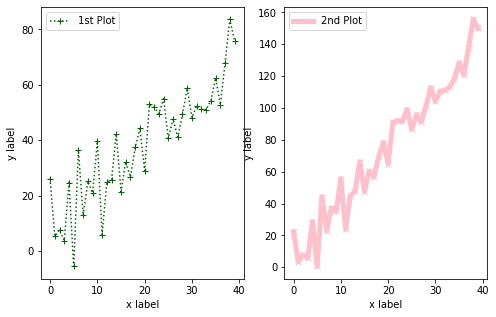
\includegraphics[width=0.65\textwidth]{figures/matplotlib_25_0.png}
\end{figure}

Subplots can also be arranged in another way like

\begin{tcolorbox}[breakable, size=fbox, boxrule=1pt, pad at break*=1mm,colback=cellbackground, colframe=cellborder]
\begin{Verbatim}[commandchars=\\\{\}]
\PY{n}{fig} \PY{o}{=} \PY{n}{plt}\PY{o}{.}\PY{n}{figure}\PY{p}{(}\PY{n}{figsize}\PY{o}{=}\PY{p}{(}\PY{l+m+mi}{8}\PY{p}{,}\PY{l+m+mi}{5}\PY{p}{)}\PY{p}{)}
	
\PY{n}{sub1} \PY{o}{=} \PY{n}{plt}\PY{o}{.}\PY{n}{subplot}\PY{p}{(}\PY{l+m+mi}{2}\PY{p}{,} \PY{l+m+mi}{1}\PY{p}{,} \PY{l+m+mi}{1}\PY{p}{)}
\PY{n}{sub1}\PY{o}{.}\PY{n}{plot}\PY{p}{(}\PY{n}{x}\PY{p}{,} \PY{n}{y1}\PY{p}{,} \PY{n}{marker}\PY{o}{=}\PY{l+s+s2}{\PYZdq{}}\PY{l+s+s2}{+}\PY{l+s+s2}{\PYZdq{}}\PY{p}{,} \PY{n}{linestyle}\PY{o}{=}\PY{l+s+s2}{\PYZdq{}}\PY{l+s+s2}{:}\PY{l+s+s2}{\PYZdq{}}\PY{p}{,} \PY{n}{color}\PY{o}{=}\PY{l+s+s2}{\PYZdq{}}\PY{l+s+s2}{darkgreen}\PY{l+s+s2}{\PYZdq{}}\PY{p}{,} \PY{n}{label}\PY{o}{=}\PY{l+s+s2}{\PYZdq{}}\PY{l+s+s2}{1st Plot}\PY{l+s+s2}{\PYZdq{}}\PY{p}{)}
\PY{n}{sub1}\PY{o}{.}\PY{n}{set\PYZus{}xlabel}\PY{p}{(}\PY{l+s+s2}{\PYZdq{}}\PY{l+s+s2}{x label}\PY{l+s+s2}{\PYZdq{}}\PY{p}{)}
\PY{n}{sub1}\PY{o}{.}\PY{n}{set\PYZus{}ylabel}\PY{p}{(}\PY{l+s+s2}{\PYZdq{}}\PY{l+s+s2}{y label}\PY{l+s+s2}{\PYZdq{}}\PY{p}{)}
\PY{n}{sub1}\PY{o}{.}\PY{n}{legend}\PY{p}{(}\PY{p}{)}
	
\PY{n}{sub2} \PY{o}{=} \PY{n}{plt}\PY{o}{.}\PY{n}{subplot}\PY{p}{(}\PY{l+m+mi}{2}\PY{p}{,} \PY{l+m+mi}{1}\PY{p}{,} \PY{l+m+mi}{2}\PY{p}{)}
\PY{n}{sub2}\PY{o}{.}\PY{n}{plot}\PY{p}{(}\PY{n}{x}\PY{p}{,} \PY{n}{y2}\PY{p}{,} \PY{n}{marker}\PY{o}{=}\PY{l+s+s2}{\PYZdq{}}\PY{l+s+s2}{x}\PY{l+s+s2}{\PYZdq{}}\PY{p}{,} \PY{n}{linewidth}\PY{o}{=}\PY{l+m+mi}{5}\PY{p}{,} \PY{n}{color}\PY{o}{=}\PY{l+s+s2}{\PYZdq{}}\PY{l+s+s2}{pink}\PY{l+s+s2}{\PYZdq{}}\PY{p}{,} \PY{n}{label}\PY{o}{=}\PY{l+s+s2}{\PYZdq{}}\PY{l+s+s2}{2nd Plot}\PY{l+s+s2}{\PYZdq{}}\PY{p}{)}
\PY{n}{sub2}\PY{o}{.}\PY{n}{set\PYZus{}xlabel}\PY{p}{(}\PY{l+s+s2}{\PYZdq{}}\PY{l+s+s2}{x label}\PY{l+s+s2}{\PYZdq{}}\PY{p}{)}
\PY{n}{sub2}\PY{o}{.}\PY{n}{set\PYZus{}ylabel}\PY{p}{(}\PY{l+s+s2}{\PYZdq{}}\PY{l+s+s2}{y label}\PY{l+s+s2}{\PYZdq{}}\PY{p}{)}
\PY{n}{sub2}\PY{o}{.}\PY{n}{legend}\PY{p}{(}\PY{p}{)}
	
\PY{n}{plt}\PY{o}{.}\PY{n}{show}\PY{p}{(}\PY{p}{)}
\end{Verbatim}
\end{tcolorbox}

\begin{figure}[h]
	\centering
	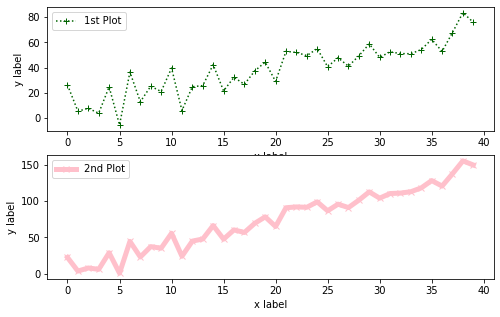
\includegraphics[width=0.65\textwidth]{figures/matplotlib_27_0.png}
\end{figure}

\subsection{Lines and Text}\label{lines-and-text}

To make plots more informative it can be useful to add text or lines on
a plot.

\subsubsection{Lines}\label{lines}

Lines can be drawn with \(\tt{hlines}\) (for horizontal lines) and
\(\tt{hvines}\) (for vertical lines). Both commands take in input the
\(y\), \(x_{min}\), \(x_{max}\) and \(x\), \(y_{min}\), \(y_{max}\)
respectively. Beware, coordinates are relative to the axis scale.

Other parameters allow to format the line in terms of color, style,
width\(\ldots\).

\begin{tcolorbox}[breakable, size=fbox, boxrule=1pt, pad at break*=1mm,colback=cellbackground, colframe=cellborder]
\begin{Verbatim}[commandchars=\\\{\}]
\PY{n}{fig} \PY{o}{=} \PY{n}{plt}\PY{o}{.}\PY{n}{figure}\PY{p}{(}\PY{n}{figsize}\PY{o}{=}\PY{p}{(}\PY{l+m+mi}{8}\PY{p}{,}\PY{l+m+mi}{5}\PY{p}{)}\PY{p}{)}
\PY{n}{plt}\PY{o}{.}\PY{n}{plot}\PY{p}{(}\PY{n}{x}\PY{p}{,} \PY{n}{y1}\PY{p}{,} \PY{n}{marker}\PY{o}{=}\PY{l+s+s2}{\PYZdq{}}\PY{l+s+s2}{+}\PY{l+s+s2}{\PYZdq{}}\PY{p}{,} \PY{n}{linestyle}\PY{o}{=}\PY{l+s+s2}{\PYZdq{}}\PY{l+s+s2}{:}\PY{l+s+s2}{\PYZdq{}}\PY{p}{,} \PY{n}{color}\PY{o}{=}\PY{l+s+s2}{\PYZdq{}}\PY{l+s+s2}{darkgreen}\PY{l+s+s2}{\PYZdq{}}\PY{p}{,} \PY{n}{label}\PY{o}{=}\PY{l+s+s2}{\PYZdq{}}\PY{l+s+s2}{1st Plot}\PY{l+s+s2}{\PYZdq{}}\PY{p}{)}
\PY{n}{plt}\PY{o}{.}\PY{n}{plot}\PY{p}{(}\PY{n}{x}\PY{p}{,} \PY{n}{y2}\PY{p}{,} \PY{n}{marker}\PY{o}{=}\PY{l+s+s2}{\PYZdq{}}\PY{l+s+s2}{x}\PY{l+s+s2}{\PYZdq{}}\PY{p}{,} \PY{n}{linewidth}\PY{o}{=}\PY{l+m+mi}{5}\PY{p}{,} \PY{n}{color}\PY{o}{=}\PY{l+s+s2}{\PYZdq{}}\PY{l+s+s2}{pink}\PY{l+s+s2}{\PYZdq{}}\PY{p}{,} \PY{n}{label}\PY{o}{=}\PY{l+s+s2}{\PYZdq{}}\PY{l+s+s2}{2nd Plot}\PY{l+s+s2}{\PYZdq{}}\PY{p}{)}
\PY{n}{plt}\PY{o}{.}\PY{n}{title}\PY{p}{(}\PY{l+s+s2}{\PYZdq{}}\PY{l+s+s2}{Plot Title}\PY{l+s+s2}{\PYZdq{}}\PY{p}{)}
\PY{n}{plt}\PY{o}{.}\PY{n}{xlabel}\PY{p}{(}\PY{l+s+s2}{\PYZdq{}}\PY{l+s+s2}{x label}\PY{l+s+s2}{\PYZdq{}}\PY{p}{)}
\PY{n}{plt}\PY{o}{.}\PY{n}{ylabel}\PY{p}{(}\PY{l+s+s2}{\PYZdq{}}\PY{l+s+s2}{y label}\PY{l+s+s2}{\PYZdq{}}\PY{p}{)}
\PY{n}{plt}\PY{o}{.}\PY{n}{hlines}\PY{p}{(}\PY{l+m+mi}{65}\PY{p}{,} \PY{l+m+mi}{0}\PY{p}{,} \PY{l+m+mf}{37.5}\PY{p}{,} \PY{n}{color}\PY{o}{=}\PY{l+s+s1}{\PYZsq{}}\PY{l+s+s1}{red}\PY{l+s+s1}{\PYZsq{}}\PY{p}{,} \PY{n}{linestyle}\PY{o}{=}\PY{l+s+s2}{\PYZdq{}}\PY{l+s+s2}{\PYZhy{}.}\PY{l+s+s2}{\PYZdq{}}\PY{p}{,} \PY{n}{label}\PY{o}{=}\PY{l+s+s1}{\PYZsq{}}\PY{l+s+s1}{Critical Thr.}\PY{l+s+s1}{\PYZsq{}}\PY{p}{)}
\PY{n}{plt}\PY{o}{.}\PY{n}{legend}\PY{p}{(}\PY{p}{)}
\PY{n}{plt}\PY{o}{.}\PY{n}{show}\PY{p}{(}\PY{p}{)}
\end{Verbatim}
\end{tcolorbox}

\begin{figure}[h]
	\centering
	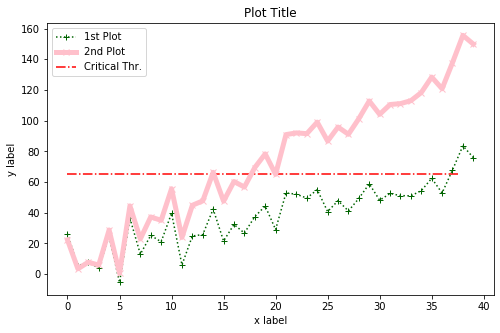
\includegraphics[width=0.7\textwidth]{figures/matplotlib_29_0.png}
\end{figure}

Notice as the \(y\) value is 65 and \(x\) goes from 0 to 37.5 which
corresponds to each axis.

Analogously for a vertical line, except that we have to first specify
the \(x\) value and then the \(y\) range.

\begin{tcolorbox}[breakable, size=fbox, boxrule=1pt, pad at break*=1mm,colback=cellbackground, colframe=cellborder]
\begin{Verbatim}[commandchars=\\\{\}]
\PY{n}{fig} \PY{o}{=} \PY{n}{plt}\PY{o}{.}\PY{n}{figure}\PY{p}{(}\PY{n}{figsize}\PY{o}{=}\PY{p}{(}\PY{l+m+mi}{8}\PY{p}{,}\PY{l+m+mi}{5}\PY{p}{)}\PY{p}{)}
\PY{n}{plt}\PY{o}{.}\PY{n}{plot}\PY{p}{(}\PY{n}{x}\PY{p}{,} \PY{n}{y1}\PY{p}{,} \PY{n}{marker}\PY{o}{=}\PY{l+s+s2}{\PYZdq{}}\PY{l+s+s2}{+}\PY{l+s+s2}{\PYZdq{}}\PY{p}{,} \PY{n}{linestyle}\PY{o}{=}\PY{l+s+s2}{\PYZdq{}}\PY{l+s+s2}{:}\PY{l+s+s2}{\PYZdq{}}\PY{p}{,} \PY{n}{color}\PY{o}{=}\PY{l+s+s2}{\PYZdq{}}\PY{l+s+s2}{darkgreen}\PY{l+s+s2}{\PYZdq{}}\PY{p}{,} \PY{n}{label}\PY{o}{=}\PY{l+s+s2}{\PYZdq{}}\PY{l+s+s2}{1st Plot}\PY{l+s+s2}{\PYZdq{}}\PY{p}{)}
\PY{n}{plt}\PY{o}{.}\PY{n}{plot}\PY{p}{(}\PY{n}{x}\PY{p}{,} \PY{n}{y2}\PY{p}{,} \PY{n}{marker}\PY{o}{=}\PY{l+s+s2}{\PYZdq{}}\PY{l+s+s2}{x}\PY{l+s+s2}{\PYZdq{}}\PY{p}{,} \PY{n}{linewidth}\PY{o}{=}\PY{l+m+mi}{5}\PY{p}{,} \PY{n}{color}\PY{o}{=}\PY{l+s+s2}{\PYZdq{}}\PY{l+s+s2}{pink}\PY{l+s+s2}{\PYZdq{}}\PY{p}{,} \PY{n}{label}\PY{o}{=}\PY{l+s+s2}{\PYZdq{}}\PY{l+s+s2}{2nd Plot}\PY{l+s+s2}{\PYZdq{}}\PY{p}{)}
\PY{n}{plt}\PY{o}{.}\PY{n}{title}\PY{p}{(}\PY{l+s+s2}{\PYZdq{}}\PY{l+s+s2}{Plot Title}\PY{l+s+s2}{\PYZdq{}}\PY{p}{)}
\PY{n}{plt}\PY{o}{.}\PY{n}{xlabel}\PY{p}{(}\PY{l+s+s2}{\PYZdq{}}\PY{l+s+s2}{x label}\PY{l+s+s2}{\PYZdq{}}\PY{p}{)}
\PY{n}{plt}\PY{o}{.}\PY{n}{ylabel}\PY{p}{(}\PY{l+s+s2}{\PYZdq{}}\PY{l+s+s2}{y label}\PY{l+s+s2}{\PYZdq{}}\PY{p}{)}
\PY{n}{plt}\PY{o}{.}\PY{n}{vlines}\PY{p}{(}\PY{l+m+mi}{22}\PY{p}{,} \PY{l+m+mi}{0}\PY{p}{,} \PY{l+m+mi}{120}\PY{p}{,} \PY{n}{color}\PY{o}{=}\PY{l+s+s1}{\PYZsq{}}\PY{l+s+s1}{gray}\PY{l+s+s1}{\PYZsq{}}\PY{p}{,} \PY{n}{label}\PY{o}{=}\PY{l+s+s1}{\PYZsq{}}\PY{l+s+s1}{Splitting Thr.}\PY{l+s+s1}{\PYZsq{}}\PY{p}{)}
\PY{n}{plt}\PY{o}{.}\PY{n}{legend}\PY{p}{(}\PY{p}{)}
\PY{n}{plt}\PY{o}{.}\PY{n}{show}\PY{p}{(}\PY{p}{)}
\end{Verbatim}
\end{tcolorbox}

\begin{figure}[h]
	\centering
	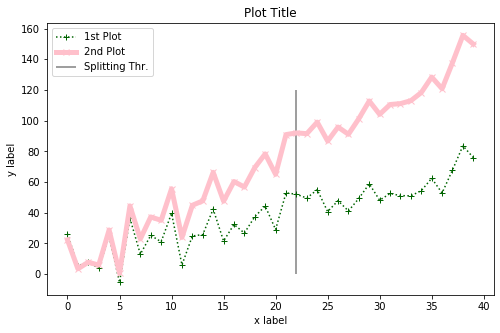
\includegraphics[width=0.7\textwidth]{figures/matplotlib_31_0.png}
\end{figure}

\subsubsection{Text}\label{text}

Like lines text can be added to the plot with the command \(\tt{text}\).
This function takes the \(x\) and \(y\) coordinates of starting point of
the text and the actual text string. Like before coordinates are
relative to the axis plot.

Other options can be used to format the text style, their meaning should
be straightforward:

\begin{itemize}
	\tightlist
	\item
	\(\tt{backgroundcolor}\);
	\item
	\(\tt{color}\);
	\item
	\(\tt{fontfamily}\): (FONTNAME, `serif', `sans-serif', `cursive',
	`fantasy', `monospace');
	\item
	\(\tt{fontsize}\); (size in points, `xx-small', `x-small', `small',
	`medium', `large', `x-large', `xx-large');
	\item
	\(\tt{fontstyle}\): (`normal', `italic', `oblique');
	\item
	\(\tt{horizontalalignment}\): (`center', `right', `left');
	\item
	\(\tt{rotation}\): takes the angle in degrees;
	\item
	\(\tt{verticalalignment}\): (`center', `top', `bottom', `baseline',
	`center\_baseline').
\end{itemize}

\begin{tcolorbox}[breakable, size=fbox, boxrule=1pt, pad at break*=1mm,colback=cellbackground, colframe=cellborder]
\begin{Verbatim}[commandchars=\\\{\}]
\PY{n}{fig} \PY{o}{=} \PY{n}{plt}\PY{o}{.}\PY{n}{figure}\PY{p}{(}\PY{n}{figsize}\PY{o}{=}\PY{p}{(}\PY{l+m+mi}{8}\PY{p}{,}\PY{l+m+mi}{5}\PY{p}{)}\PY{p}{)}
\PY{n}{plt}\PY{o}{.}\PY{n}{plot}\PY{p}{(}\PY{n}{x}\PY{p}{,} \PY{n}{y1}\PY{p}{,} \PY{n}{marker}\PY{o}{=}\PY{l+s+s2}{\PYZdq{}}\PY{l+s+s2}{+}\PY{l+s+s2}{\PYZdq{}}\PY{p}{,} \PY{n}{linestyle}\PY{o}{=}\PY{l+s+s2}{\PYZdq{}}\PY{l+s+s2}{:}\PY{l+s+s2}{\PYZdq{}}\PY{p}{,} \PY{n}{color}\PY{o}{=}\PY{l+s+s2}{\PYZdq{}}\PY{l+s+s2}{darkgreen}\PY{l+s+s2}{\PYZdq{}}\PY{p}{,} \PY{n}{label}\PY{o}{=}\PY{l+s+s2}{\PYZdq{}}\PY{l+s+s2}{1st Plot}\PY{l+s+s2}{\PYZdq{}}\PY{p}{)}
\PY{n}{plt}\PY{o}{.}\PY{n}{plot}\PY{p}{(}\PY{n}{x}\PY{p}{,} \PY{n}{y2}\PY{p}{,} \PY{n}{marker}\PY{o}{=}\PY{l+s+s2}{\PYZdq{}}\PY{l+s+s2}{x}\PY{l+s+s2}{\PYZdq{}}\PY{p}{,} \PY{n}{linewidth}\PY{o}{=}\PY{l+m+mi}{5}\PY{p}{,} \PY{n}{color}\PY{o}{=}\PY{l+s+s2}{\PYZdq{}}\PY{l+s+s2}{pink}\PY{l+s+s2}{\PYZdq{}}\PY{p}{,} \PY{n}{label}\PY{o}{=}\PY{l+s+s2}{\PYZdq{}}\PY{l+s+s2}{2nd Plot}\PY{l+s+s2}{\PYZdq{}}\PY{p}{)}
\PY{n}{plt}\PY{o}{.}\PY{n}{title}\PY{p}{(}\PY{l+s+s2}{\PYZdq{}}\PY{l+s+s2}{Plot Title}\PY{l+s+s2}{\PYZdq{}}\PY{p}{)}
\PY{n}{plt}\PY{o}{.}\PY{n}{xlabel}\PY{p}{(}\PY{l+s+s2}{\PYZdq{}}\PY{l+s+s2}{x label}\PY{l+s+s2}{\PYZdq{}}\PY{p}{)}
\PY{n}{plt}\PY{o}{.}\PY{n}{ylabel}\PY{p}{(}\PY{l+s+s2}{\PYZdq{}}\PY{l+s+s2}{y label}\PY{l+s+s2}{\PYZdq{}}\PY{p}{)}
\PY{n}{plt}\PY{o}{.}\PY{n}{vlines}\PY{p}{(}\PY{l+m+mi}{22}\PY{p}{,} \PY{l+m+mi}{0}\PY{p}{,} \PY{l+m+mi}{120}\PY{p}{,} \PY{n}{color}\PY{o}{=}\PY{l+s+s1}{\PYZsq{}}\PY{l+s+s1}{gray}\PY{l+s+s1}{\PYZsq{}}\PY{p}{)}
\PY{n}{plt}\PY{o}{.}\PY{n}{text}\PY{p}{(}\PY{l+m+mi}{23}\PY{p}{,} \PY{l+m+mi}{5}\PY{p}{,} \PY{l+s+s2}{\PYZdq{}}\PY{l+s+s2}{Splitting Thr.}\PY{l+s+s2}{\PYZdq{}}\PY{p}{,} \PY{n}{rotation}\PY{o}{=}\PY{l+m+mi}{90}\PY{p}{)}
\PY{n}{plt}\PY{o}{.}\PY{n}{hlines}\PY{p}{(}\PY{l+m+mi}{65}\PY{p}{,} \PY{l+m+mi}{0}\PY{p}{,} \PY{l+m+mf}{37.5}\PY{p}{,} \PY{n}{color}\PY{o}{=}\PY{l+s+s1}{\PYZsq{}}\PY{l+s+s1}{red}\PY{l+s+s1}{\PYZsq{}}\PY{p}{,} \PY{n}{linestyle}\PY{o}{=}\PY{l+s+s2}{\PYZdq{}}\PY{l+s+s2}{\PYZhy{}.}\PY{l+s+s2}{\PYZdq{}}\PY{p}{)}
\PY{n}{plt}\PY{o}{.}\PY{n}{text}\PY{p}{(}\PY{l+m+mi}{25}\PY{p}{,} \PY{l+m+mi}{75}\PY{p}{,} \PY{l+s+s2}{\PYZdq{}}\PY{l+s+s2}{Critical Thr.}\PY{l+s+s2}{\PYZdq{}}\PY{p}{,} \PY{n}{backgroundcolor}\PY{o}{=}\PY{l+s+s2}{\PYZdq{}}\PY{l+s+s2}{red}\PY{l+s+s2}{\PYZdq{}}\PY{p}{,} \PY{n}{color}\PY{o}{=}\PY{l+s+s2}{\PYZdq{}}\PY{l+s+s2}{white}\PY{l+s+s2}{\PYZdq{}}\PY{p}{)}
\PY{n}{plt}\PY{o}{.}\PY{n}{legend}\PY{p}{(}\PY{p}{)}
\PY{n}{plt}\PY{o}{.}\PY{n}{show}\PY{p}{(}\PY{p}{)}
\end{Verbatim}
\end{tcolorbox}

\begin{figure}[h]
	\centering
	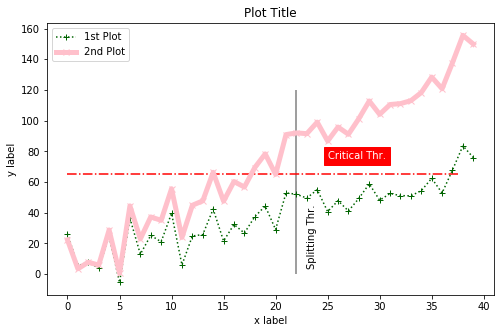
\includegraphics[width=0.7\textwidth]{figures/matplotlib_33_0.png}
\end{figure}

\subsection{Saving}\label{saving}

A plot can be saved into a file for later usage with \(\tt{savefig}\)
which takes in input the file name. The format of the file will be
inferred from the file name extension (.jpg, .png, .gif\ldots{})

\begin{tcolorbox}[breakable, size=fbox, boxrule=1pt, pad at break*=1mm,colback=cellbackground, colframe=cellborder]
\begin{Verbatim}[commandchars=\\\{\}]
\PY{n}{plt}\PY{o}{.}\PY{n}{savefig}\PY{p}{(}\PY{l+s+s2}{\PYZdq{}}\PY{l+s+s2}{myfigure.png}\PY{l+s+s2}{\PYZdq{}}\PY{p}{)}
\end{Verbatim}
\end{tcolorbox}

%\subsection{Plot a graph given \(x\) and \(y\) values (scatter-plot)}\label{plot-a-graph-given-x-and-y-values}
%
%\begin{tcolorbox}[breakable, size=fbox, boxrule=1pt, pad at break*=1mm,colback=cellbackground, colframe=cellborder]
%\begin{Verbatim}[commandchars=\\\{\}]
%\PY{k+kn}{from} \PY{n+nn}{matplotlib} \PY{k}{import} \PY{n}{pyplot} \PY{k}{as} \PY{n}{plt}
%
%\PY{n}{x} \PY{o}{=} \PY{p}{[}\PY{l+m+mi}{1}\PY{p}{,} \PY{l+m+mi}{2}\PY{p}{,} \PY{l+m+mi}{3}\PY{p}{]}
%\PY{n}{y} \PY{o}{=} \PY{p}{[}\PY{l+m+mf}{0.3}\PY{p}{,} \PY{l+m+mf}{0.4}\PY{p}{,} \PY{l+m+mf}{0.6}\PY{p}{]}
% 
%\PY{n}{plt}\PY{o}{.}\PY{n}{plot}\PY{p}{(}\PY{n}{x}\PY{p}{,} \PY{n}{y}\PY{p}{,} \PY{n}{marker}\PY{o}{=}\PY{l+s+s1}{\PYZsq{}}\PY{l+s+s1}{o}\PY{l+s+s1}{\PYZsq{}}\PY{p}{)} \PY{c+c1}{\PYZsh{} we are using circle markers}
%\PY{n}{plt}\PY{o}{.}\PY{n}{grid}\PY{p}{(}\PY{k+kc}{True}\PY{p}{)}               \PY{c+c1}{\PYZsh{} this line activate grid drawing}
%\PY{n}{plt}\PY{o}{.}\PY{n}{show}\PY{p}{(}\PY{p}{)}
%\end{Verbatim}
%\end{tcolorbox}
%
%\begin{figure}[h]
%\centering
%  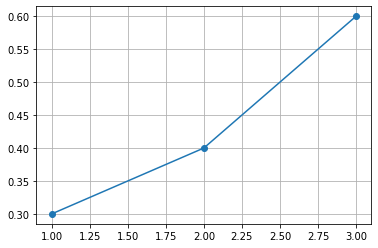
\includegraphics[width=0.6\textwidth]{figures/Untitled_43_0.png}
%\end{figure}
%%    { \hspace*{\fill} \\}
%    
%\begin{tcolorbox}[breakable, size=fbox, boxrule=1pt, pad at break*=1mm,colback=cellbackground, colframe=cellborder]
%\begin{Verbatim}[commandchars=\\\{\}]
%\PY{c+c1}{\PYZsh{} if we want to plot specific points too}
%
%\PY{n}{x} \PY{o}{=} \PY{p}{[}\PY{l+m+mi}{1}\PY{p}{,} \PY{l+m+mi}{2}\PY{p}{,} \PY{l+m+mi}{3}\PY{p}{]}
%\PY{n}{y} \PY{o}{=} \PY{p}{[}\PY{l+m+mf}{0.3}\PY{p}{,} \PY{l+m+mf}{0.4}\PY{p}{,} \PY{l+m+mf}{0.6}\PY{p}{]}
% 
%\PY{n}{plt}\PY{o}{.}\PY{n}{plot}\PY{p}{(}\PY{n}{x}\PY{p}{,} \PY{n}{y}\PY{p}{,} \PY{n}{marker}\PY{o}{=}\PY{l+s+s1}{\PYZsq{}}\PY{l+s+s1}{x}\PY{l+s+s1}{\PYZsq{}}\PY{p}{)}
%\PY{n}{plt}\PY{o}{.}\PY{n}{plot}\PY{p}{(}\PY{l+m+mf}{2.5}\PY{p}{,} \PY{l+m+mf}{0.5}\PY{p}{,} \PY{n}{marker}\PY{o}{=}\PY{l+s+s1}{\PYZsq{}}\PY{l+s+s1}{X}\PY{l+s+s1}{\PYZsq{}}\PY{p}{,} \PY{n}{ms}\PY{o}{=}\PY{l+m+mi}{12}\PY{p}{,} \PY{n}{color}\PY{o}{=}\PY{l+s+s1}{\PYZsq{}}\PY{l+s+s1}{red}\PY{l+s+s1}{\PYZsq{}}\PY{p}{)}
%\PY{n}{plt}\PY{o}{.}\PY{n}{plot}\PY{p}{(}\PY{l+m+mf}{1.5}\PY{p}{,} \PY{l+m+mf}{0.35}\PY{p}{,} \PY{n}{marker}\PY{o}{=}\PY{l+s+s1}{\PYZsq{}}\PY{l+s+s1}{x}\PY{l+s+s1}{\PYZsq{}}\PY{p}{,} \PY{n}{ms}\PY{o}{=}\PY{l+m+mi}{12}\PY{p}{,} \PY{n}{color}\PY{o}{=}\PY{l+s+s1}{\PYZsq{}}\PY{l+s+s1}{red}\PY{l+s+s1}{\PYZsq{}}\PY{p}{)}
%\PY{n}{plt}\PY{o}{.}\PY{n}{grid}\PY{p}{(}\PY{k+kc}{True}\PY{p}{)}              
%\PY{n}{plt}\PY{o}{.}\PY{n}{show}\PY{p}{(}\PY{p}{)}
%\end{Verbatim}
%\end{tcolorbox}
%
%\begin{figure}[h]
%\centering
%  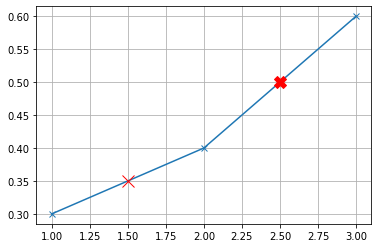
\includegraphics[width=0.6\textwidth]{figures/Untitled_44_0.png}
%\end{figure}
%%    { \hspace*{\fill} \\}
%    
%\subsubsection{What if \(x\) values are dates ?}
%
%\begin{tcolorbox}[breakable, size=fbox, boxrule=1pt, pad at break*=1mm,colback=cellbackground, colframe=cellborder]
%\begin{Verbatim}[commandchars=\\\{\}]
%\PY{k+kn}{import} \PY{n+nn}{datetime}
%\PY{k+kn}{import} \PY{n+nn}{matplotlib}\PY{n+nn}{.}\PY{n+nn}{dates} \PY{k}{as} \PY{n+nn}{mdates}
%
%\PY{n}{x} \PY{o}{=} \PY{p}{[}\PY{n}{datetime}\PY{o}{.}\PY{n}{date}\PY{p}{(}\PY{l+m+mi}{2020}\PY{p}{,} \PY{l+m+mi}{7}\PY{p}{,} \PY{l+m+mi}{20}\PY{p}{)}\PY{p}{,}  \PY{n}{datetime}\PY{o}{.}\PY{n}{date}\PY{p}{(}\PY{l+m+mi}{2020}\PY{p}{,} \PY{l+m+mi}{7}\PY{p}{,} \PY{l+m+mi}{30}\PY{p}{)}\PY{p}{,} 
%     \PY{n}{datetime}\PY{o}{.}\PY{n}{date}\PY{p}{(}\PY{l+m+mi}{2020}\PY{p}{,} \PY{l+m+mi}{8}\PY{p}{,} \PY{l+m+mi}{10}\PY{p}{)}\PY{p}{,}  \PY{n}{datetime}\PY{o}{.}\PY{n}{date}\PY{p}{(}\PY{l+m+mi}{2020}\PY{p}{,} \PY{l+m+mi}{8}\PY{p}{,} \PY{l+m+mi}{20}\PY{p}{)}\PY{p}{]}
%     
%\PY{n}{y} \PY{o}{=} \PY{p}{[}\PY{l+m+mi}{10}\PY{p}{,} \PY{l+m+mi}{20}\PY{p}{,} \PY{l+m+mi}{34}\PY{p}{,} \PY{l+m+mi}{45}\PY{p}{]}
%\PY{n}{plt}\PY{o}{.}\PY{n}{plot}\PY{p}{(}\PY{n}{x}\PY{p}{,} \PY{n}{y}\PY{p}{,} \PY{n}{marker}\PY{o}{=}\PY{l+s+s1}{\PYZsq{}}\PY{l+s+s1}{o}\PY{l+s+s1}{\PYZsq{}}\PY{p}{)}
%\PY{c+c1}{\PYZsh{} this line tells matplotlib we have dates on x axis}
%\PY{n}{plt}\PY{o}{.}\PY{n}{gca}\PY{p}{(}\PY{p}{)}\PY{o}{.}\PY{n}{xaxis}\PY{o}{.}\PY{n}{set\PYZus{}major\PYZus{}formatter}\PY{p}{(}\PY{n}{mdates}\PY{o}{.}\PY{n}{DateFormatter}\PY{p}{(}\PY{l+s+s1}{\PYZsq{}}\PY{l+s+s1}{\PYZpc{}}\PY{l+s+s1}{Y\PYZhy{}}\PY{l+s+s1}{\PYZpc{}}\PY{l+s+s1}{m\PYZhy{}}\PY{l+s+si}{\PYZpc{}d}\PY{l+s+s1}{\PYZsq{}}\PY{p}{)}\PY{p}{)}
%\PY{c+c1}{\PYZsh{} this one instead rotate labels to avoid superimposition}
%\PY{n}{plt}\PY{o}{.}\PY{n}{xticks}\PY{p}{(}\PY{n}{rotation}\PY{o}{=}\PY{l+m+mi}{45}\PY{p}{)}
%\PY{n}{plt}\PY{o}{.}\PY{n}{grid}\PY{p}{(}\PY{k+kc}{True}\PY{p}{)}
%\PY{n}{plt}\PY{o}{.}\PY{n}{show}\PY{p}{(}\PY{p}{)}
%\end{Verbatim}
%\end{tcolorbox}
%
%\begin{figure}[h]
%\centering
%  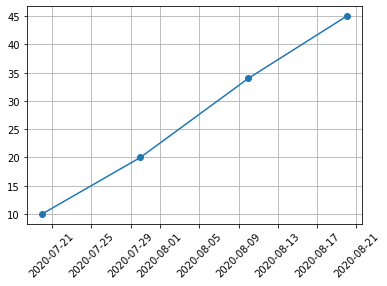
\includegraphics[width=0.6\textwidth]{figures/Untitled_46_0.png}
%\end{figure}
%%    { \hspace*{\fill} \\}
%    
%\subsection{Plotting an Histogram}\label{plotting-an-histogram}
%
%\begin{tcolorbox}[breakable, size=fbox, boxrule=1pt, pad at break*=1mm,colback=cellbackground, colframe=cellborder]
%\begin{Verbatim}[commandchars=\\\{\}]
%\PY{k+kn}{import} \PY{n+nn}{random} 
%\PY{n}{numbers} \PY{o}{=} \PY{p}{[}\PY{p}{]}
%\PY{k}{for} \PY{n}{\PYZus{}} \PY{o+ow}{in} \PY{n+nb}{range}\PY{p}{(}\PY{l+m+mi}{1000}\PY{p}{)}\PY{p}{:}
%  \PY{n}{numbers}\PY{o}{.}\PY{n}{append}\PY{p}{(}\PY{n}{random}\PY{o}{.}\PY{n}{randint}\PY{p}{(}\PY{l+m+mi}{1}\PY{p}{,} \PY{l+m+mi}{10}\PY{p}{)}\PY{p}{)}
%
%\PY{k+kn}{from} \PY{n+nn}{matplotlib} \PY{k}{import} \PY{n}{pyplot} \PY{k}{as} \PY{n}{plt}
%
%\PY{c+c1}{\PYZsh{} Here we define the binning}
%\PY{c+c1}{\PYZsh{} 6 is the number of bins, going from 0 to 10}
%\PY{n}{plt}\PY{o}{.}\PY{n}{hist}\PY{p}{(}\PY{n}{numbers}\PY{p}{,} \PY{l+m+mi}{10}\PY{p}{,} \PY{n+nb}{range}\PY{o}{=}\PY{p}{[}\PY{l+m+mi}{0}\PY{p}{,} \PY{l+m+mi}{11}\PY{p}{]}\PY{p}{)} 
%\PY{n}{plt}\PY{o}{.}\PY{n}{show}\PY{p}{(}\PY{p}{)}
%\end{Verbatim}
%\end{tcolorbox}
%
%\begin{figure}[h]
%\centering
%  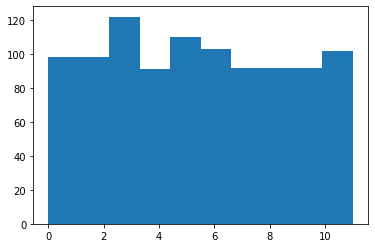
\includegraphics[width=0.55\textwidth]{figures/Untitled_48_0.png}
%\end{figure}
% %   { \hspace*{\fill} \\}
%    
%\subsubsection{Plotting a Function}\label{plotting-a-function}
%
%In this case let's try to make the plot prettier adding labels, legend\ldots{}
%All the commands apply also to the previous examples.
%
%\begin{tcolorbox}[breakable, size=fbox, boxrule=1pt, pad at break*=1mm,colback=cellbackground, colframe=cellborder]
%\begin{Verbatim}[commandchars=\\\{\}]
%\PY{k+kn}{import} \PY{n+nn}{numpy} \PY{k}{as} \PY{n+nn}{np}
%\PY{k+kn}{import} \PY{n+nn}{matplotlib}\PY{n+nn}{.}\PY{n+nn}{pyplot} \PY{k}{as} \PY{n+nn}{plt}
%\PY{k+kn}{from} \PY{n+nn}{scipy}\PY{n+nn}{.}\PY{n+nn}{stats} \PY{k}{import} \PY{n}{norm}
%
%\PY{c+c1}{\PYZsh{} define the functions to plot}
%\PY{c+c1}{\PYZsh{} a gaussian with mean=0  and sigma=1}
%\PY{c+c1}{\PYZsh{} in scipy module this is called norm}
%\PY{n}{mu}\PY{o}{=}\PY{l+m+mi}{0}
%\PY{n}{sigma} \PY{o}{=} \PY{l+m+mi}{1}
%\PY{n}{x} \PY{o}{=} \PY{n}{np}\PY{o}{.}\PY{n}{arange}\PY{p}{(}\PY{o}{\PYZhy{}}\PY{l+m+mi}{10}\PY{p}{,} \PY{o}{\PYZhy{}}\PY{l+m+mf}{1.645}\PY{p}{,} \PY{l+m+mf}{0.001}\PY{p}{)}
%\PY{n}{x\PYZus{}all} \PY{o}{=} \PY{n}{np}\PY{o}{.}\PY{n}{arange}\PY{p}{(}\PY{o}{\PYZhy{}}\PY{l+m+mi}{4}\PY{p}{,} \PY{l+m+mi}{4}\PY{p}{,} \PY{l+m+mf}{0.001}\PY{p}{)}
%\PY{n}{y} \PY{o}{=} \PY{n}{norm}\PY{o}{.}\PY{n}{pdf}\PY{p}{(}\PY{n}{x}\PY{p}{,} \PY{l+m+mi}{0}\PY{p}{,} \PY{l+m+mi}{1}\PY{p}{)}
%\PY{n}{y\PYZus{}all} \PY{o}{=} \PY{n}{norm}\PY{o}{.}\PY{n}{pdf}\PY{p}{(}\PY{n}{x\PYZus{}all}\PY{p}{,} \PY{l+m+mi}{0}\PY{p}{,} \PY{l+m+mi}{1}\PY{p}{)}
%
%\PY{c+c1}{\PYZsh{} draw the gaussian}
%\PY{n}{plt}\PY{o}{.}\PY{n}{plot}\PY{p}{(}\PY{n}{x\PYZus{}all}\PY{p}{,} \PY{n}{y\PYZus{}all}\PY{p}{,} \PY{n}{label}\PY{o}{=}\PY{l+s+s1}{\PYZsq{}}\PY{l+s+s1}{Gaussian}\PY{l+s+s1}{\PYZsq{}}\PY{p}{)}
%
%\PY{c+c1}{\PYZsh{} fill with different alpha using x\PYZus{}all and y\PYZus{}all as limits}
%\PY{c+c1}{\PYZsh{} alpha set the transparency level: 0 trasparent, 1 solid}
%\PY{n}{plt}\PY{o}{.}\PY{n}{fill\PYZus{}between}\PY{p}{(}\PY{n}{x\PYZus{}all}\PY{p}{,} \PY{n}{y\PYZus{}all}\PY{p}{,} \PY{l+m+mi}{0}\PY{p}{,} \PY{n}{alpha}\PY{o}{=}\PY{l+m+mf}{0.1}\PY{p}{,} \PY{n}{color}\PY{o}{=}\PY{l+s+s1}{\PYZsq{}}\PY{l+s+s1}{blue}\PY{l+s+s1}{\PYZsq{}}\PY{p}{,} \PY{n}{label}\PY{o}{=}\PY{l+s+s2}{\PYZdq{}}\PY{l+s+s2}{Gaussian CDF}\PY{l+s+s2}{\PYZdq{}}\PY{p}{)}
%
%\PY{c+c1}{\PYZsh{} fill with color red using x and y as limits}
%\PY{c+c1}{\PYZsh{} label associate text to the object for the legend}
%\PY{n}{plt}\PY{o}{.}\PY{n}{fill\PYZus{}between}\PY{p}{(}\PY{n}{x}\PY{p}{,} \PY{n}{y}\PY{p}{,} \PY{l+m+mi}{0}\PY{p}{,} \PY{n}{alpha}\PY{o}{=}\PY{l+m+mi}{1}\PY{p}{,} \PY{n}{color}\PY{o}{=}\PY{l+s+s1}{\PYZsq{}}\PY{l+s+s1}{red}\PY{l+s+s1}{\PYZsq{}}\PY{p}{,} \PY{n}{label}\PY{o}{=}\PY{l+s+s2}{\PYZdq{}}\PY{l+s+s2}{5}\PY{l+s+s2}{\PYZpc{}}\PY{l+s+s2}{ tail}\PY{l+s+s2}{\PYZdq{}}\PY{p}{)}
%
%\PY{c+c1}{\PYZsh{} set x axis limits}
%\PY{n}{plt}\PY{o}{.}\PY{n}{xlim}\PY{p}{(}\PY{p}{[}\PY{o}{\PYZhy{}}\PY{l+m+mi}{4}\PY{p}{,} \PY{l+m+mi}{4}\PY{p}{]}\PY{p}{)}
%
%\PY{c+c1}{\PYZsh{} add a label for X axis}
%\PY{n}{plt}\PY{o}{.}\PY{n}{xlabel}\PY{p}{(}\PY{l+s+s2}{\PYZdq{}}\PY{l+s+s2}{Changes of value}\PY{l+s+s2}{\PYZdq{}}\PY{p}{)}
%
%\PY{c+c1}{\PYZsh{} add a label to y axis}
%\PY{n}{plt}\PY{o}{.}\PY{n}{ylabel}\PY{p}{(}\PY{l+s+s2}{\PYZdq{}}\PY{l+s+s2}{Gaussian values}\PY{l+s+s2}{\PYZdq{}}\PY{p}{)}
%
%\PY{c+c1}{\PYZsh{} add histogram title}
%\PY{n}{plt}\PY{o}{.}\PY{n}{title}\PY{p}{(}\PY{l+s+s2}{\PYZdq{}}\PY{l+s+s2}{Distribution of changes of value}\PY{l+s+s2}{\PYZdq{}}\PY{p}{)}
%
%\PY{c+c1}{\PYZsh{} draw a vertical line at x=\PYZhy{}1.645}
%\PY{c+c1}{\PYZsh{} y limits are in percent w.r.t. to y axis length}
%\PY{n}{plt}\PY{o}{.}\PY{n}{axvline}\PY{p}{(}\PY{n}{x}\PY{o}{=}\PY{o}{\PYZhy{}}\PY{l+m+mf}{1.645}\PY{p}{,} \PY{n}{ymin}\PY{o}{=}\PY{l+m+mf}{0.1}\PY{p}{,} \PY{n}{ymax}\PY{o}{=}\PY{l+m+mi}{1}\PY{p}{,} \PY{n}{linestyle}\PY{o}{=}\PY{l+s+s1}{\PYZsq{}}\PY{l+s+s1}{:}\PY{l+s+s1}{\PYZsq{}}\PY{p}{,} \PY{n}{linewidth}\PY{o}{=}\PY{l+m+mi}{1}\PY{p}{,} \PY{n}{color} \PY{o}{=} \PY{l+s+s1}{\PYZsq{}}\PY{l+s+s1}{red}\PY{l+s+s1}{\PYZsq{}}\PY{p}{)}
%
%\PY{c+c1}{\PYZsh{} write some text to explain the line}
%\PY{n}{plt}\PY{o}{.}\PY{n}{text}\PY{p}{(}\PY{o}{\PYZhy{}}\PY{l+m+mf}{1.9}\PY{p}{,} \PY{o}{.}\PY{l+m+mi}{12}\PY{p}{,} \PY{l+s+s1}{\PYZsq{}}\PY{l+s+s1}{95}\PY{l+s+s1}{\PYZpc{}}\PY{l+s+s1}{ percentile (VaR loss)}\PY{l+s+s1}{\PYZsq{}}\PY{p}{,}\PY{n}{fontsize}\PY{o}{=}\PY{l+m+mi}{10}\PY{p}{,} \PY{n}{rotation}\PY{o}{=}\PY{l+m+mi}{90}\PY{p}{,} 
%                                    \PY{n}{color}\PY{o}{=}\PY{l+s+s1}{\PYZsq{}}\PY{l+s+s1}{red}\PY{l+s+s1}{\PYZsq{}}\PY{p}{)}
%
%\PY{n}{plt}\PY{o}{.}\PY{n}{legend}\PY{p}{(}\PY{p}{)}
%\PY{n}{plt}\PY{o}{.}\PY{n}{show}\PY{p}{(}\PY{p}{)}
%\end{Verbatim}
%\end{tcolorbox}
%
%\begin{figure}[htp]
%\centering
%  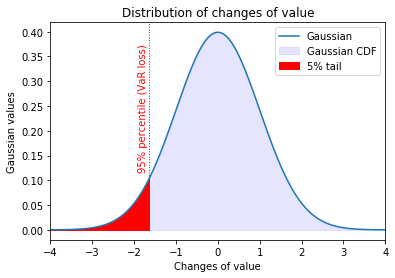
\includegraphics[width=0.55\textwidth]{figures/Untitled_50_0.png}
%\end{figure}
%%    { \hspace*{\fill} \\}
%    \clearpage
%If you are particularly satisfied by your work you can save the graph to a file:
%
%\begin{tcolorbox}[breakable, size=fbox, boxrule=1pt, pad at break*=1mm,colback=cellbackground, colframe=cellborder]
%\begin{Verbatim}[commandchars=\\\{\}]
%\PY{n}{plt}\PY{o}{.}\PY{n}{savefig}\PY{p}{(}\PY{l+s+s1}{\PYZsq{}}\PY{l+s+s1}{normal\PYZus{}curve.png}\PY{l+s+s1}{\PYZsq{}}\PY{p}{)}
%
%<Figure size 432x288 with 0 Axes>
%
%\end{Verbatim}
%\end{tcolorbox}

\begin{thebibliography}{9}
  %  %\bibitem{survey2019} StackOverflow \emph{The TEXbook}, Addison-Wesley, Reading,Massachusetts, second edition, 1984,
\bibitem{pandas} \href{https://pandas.pydata.org/docs/}{https://pandas.pydata.org/docs/}, \texttt{pandas} official documentation [Online]
\bibitem{matplotlib} \href{https://matplotlib.org}{https://matplotlib.org}, \texttt{matplotlib} official documentation [Online]
\bibitem{quandl} \href{https://docs.quandl.com/}{https://docs.quandl.com/}, \texttt{quandl} documentation [Online]
\bibitem{ffn} \href{https://pmorissette.github.io/ffn/}{https://pmorissette.github.io/ffn/}, Financial Functions for Python [Online]
\end{thebibliography}
